%%%%%%%%%%%%%%%%%%%%%%%%%%%%%%%%%%%%%%%%%
% Masters/Doctoral Thesis
% LaTeX Template
% Version 2.5 (27/8/17)
%
% This template was downloaded from:
% http://www.LaTeXTemplates.com
%
% Version 2.x major modifications by:
% Vel (vel@latextemplates.com)
%
% This template is based on a template by:
% Steve Gunn (http://users.ecs.soton.ac.uk/srg/softwaretools/document/templates/)
% Sunil Patel (http://www.sunilpatel.co.uk/thesis-template/)
%
% Template license:
% CC BY-NC-SA 3.0 (http://creativecommons.org/licenses/by-nc-sa/3.0/)
%
%%%%%%%%%%%%%%%%%%%%%%%%%%%%%%%%%%%%%%%%%

%----------------------------------------------------------------------------------------
%	PACKAGES AND OTHER DOCUMENT CONFIGURATIONS
%----------------------------------------------------------------------------------------

% Pages (from the internal page numbering) to be printed in color - 3, 4, 5, 11, 12, 13, 14, 17, 18, 20, 21, 23, 25, 27.

\documentclass[	
hidelinks, 
12pt, % The default document font size, options: 10pt, 11pt, 12pt
oneside, % Two side (alternating margins) for binding by default, uncomment to switch to one side
english, % ngerman for German
doublespacing, % Single line spacing, alternatives: onehalfspacing or singlespacing
%draft, % Uncomment to enable draft mode (no pictures, no links, overfull hboxes indicated)
%nolistspacing, % If the document is onehalfspacing or doublespacing, uncomment this to set spacing in lists to single
%liststotoc, % Uncomment to add the list of figures/tables/etc to the table of contents
%toctotoc, % Uncomment to add the main table of contents to the table of contents
%parskip, % Uncomment to add space between paragraphs
%nohyperref, % Uncomment to not load the hyperref package
headsepline, % Uncomment to get a line under the header
%chapterinoneline, % Uncomment to place the chapter title next to the number on one line
%consistentlayout, % Uncomment to change the layout of the declaration, abstract and acknowledgements pages to match the default layout
]{MastersDoctoralThesis} % The class file specifying the document structure

\usepackage[utf8]{inputenc} % Required for inputting international characters
\usepackage[T1]{fontenc} % Output font encoding for international characters
\usepackage{subcaption}
\usepackage{mathpazo} % Use the Palatino font by default
\usepackage{booktabs}
\usepackage{colortbl}
\usepackage[final]{pdfpages}
\usepackage{xcolor}
\usepackage{balance}
\usepackage{epigraph}
\usepackage{alltt} % for code snippet
\usepackage{hyperref}
\usepackage{amsmath}
\usepackage[backend=bibtex,style=authoryear,natbib=true]{biblatex} % Use the bibtex backend with the authoryear citation style (which resembles APA)
\usepackage{minted}
\usepackage{microtype}
\usepackage{url}
\DeclareRobustCommand{\code}{\texttt}
\setcounter{secnumdepth}{3}
\usemintedstyle{friendly}
\definecolor{bg}{rgb}{0.94, 0.97, 1.0}
\setminted{bgcolor=bg, breaklines=true, fontsize=\footnotesize, mathescape=false}

\addbibresource{biblio.bib} % The filename of the bibliography


\usepackage[autostyle=true]{csquotes} % Required to generate language-dependent quotes in the bibliography

%----------------------------------------------------------------------------------------
%	MARGIN SETTINGS
%----------------------------------------------------------------------------------------

\geometry{
	paper=a4paper, % Change to letterpaper for US letter
	inner=4.0cm, % Inner margin
	outer=3.0cm, % Outer margin
	bindingoffset=.5cm, % Binding offset
	top=2.5cm, % Top margin
	bottom=2.5cm, % Bottom margin
	%showframe, % Uncomment to show how the type block is set on the page
}

%----------------------------------------------------------------------------------------
%	THESIS INFORMATION
%----------------------------------------------------------------------------------------

\thesistitle{Learning Support for Writing Proofs in Coq} % Your thesis title, this is used in the title and abstract, print it elsewhere with \ttitle
\supervisor{Pr. Olivier \textsc{Danvy}} % Your supervisor's name, this is used in the title page, print it elsewhere with \supname
\examiner{Dr/Pr. FirstName \textsc{LastName}} % Your examiner's name, this is not currently used anywhere in the template, print it elsewhere with \examname
\degree{B.Sc (Hons)} % Your degree name, this is used in the title page and abstract, print it elsewhere with \degreename
\author{Jeremy \textsc{Yew}} % Your name, this is used in the title page and abstract, print it elsewhere with \authorname
\addresses{} % Your address, this is not currently used anywhere in the template, print it elsewhere with \addressname

\subject{Mathematical, Computational and Statistical Sciences} % Your subject area, this is not currently used anywhere in the template, print it elsewhere with \subjectname
\keywords{Insert, keywords, here} % Keywords for your thesis, this is not currently used anywhere in the template, print it elsewhere with \keywordnames
\university{\href{https://www.yale-nus.edu.sg/}{Yale-NUS College}} % Your university's name and URL, this is used in the title page and abstract, print it elsewhere with \univname
\department{{}} % Your department's name and URL, this is used in the title page and abstract, print it elsewhere with \deptname
\group{{}} % Your research group's name and URL, this is used in the title page, print it elsewhere with \groupname
\faculty{{}} % Your faculty's name and URL, this is used in the title page and abstract, print it elsewhere with \facname

\AtBeginDocument{
\hypersetup{colorlinks=false}
\hypersetup{pdftitle=\ttitle} % Set the PDF's title to your title
\hypersetup{pdfauthor=\authorname} % Set the PDF's author to your name
\hypersetup{pdfkeywords=\keywordnames} % Set the PDF's keywords to your keywords
}

\begin{document}

\frontmatter % Use roman page numbering style (i, ii, iii, iv...) for the pre-content pages

\pagestyle{plain} % Default to the plain heading style until the thesis style is called for the body content

%----------------------------------------------------------------------------------------
%	TITLE PAGE
%----------------------------------------------------------------------------------------

\begin{titlepage}
	% Fill out the titlepage.docx document, then save it as a pdf for inclusion here
	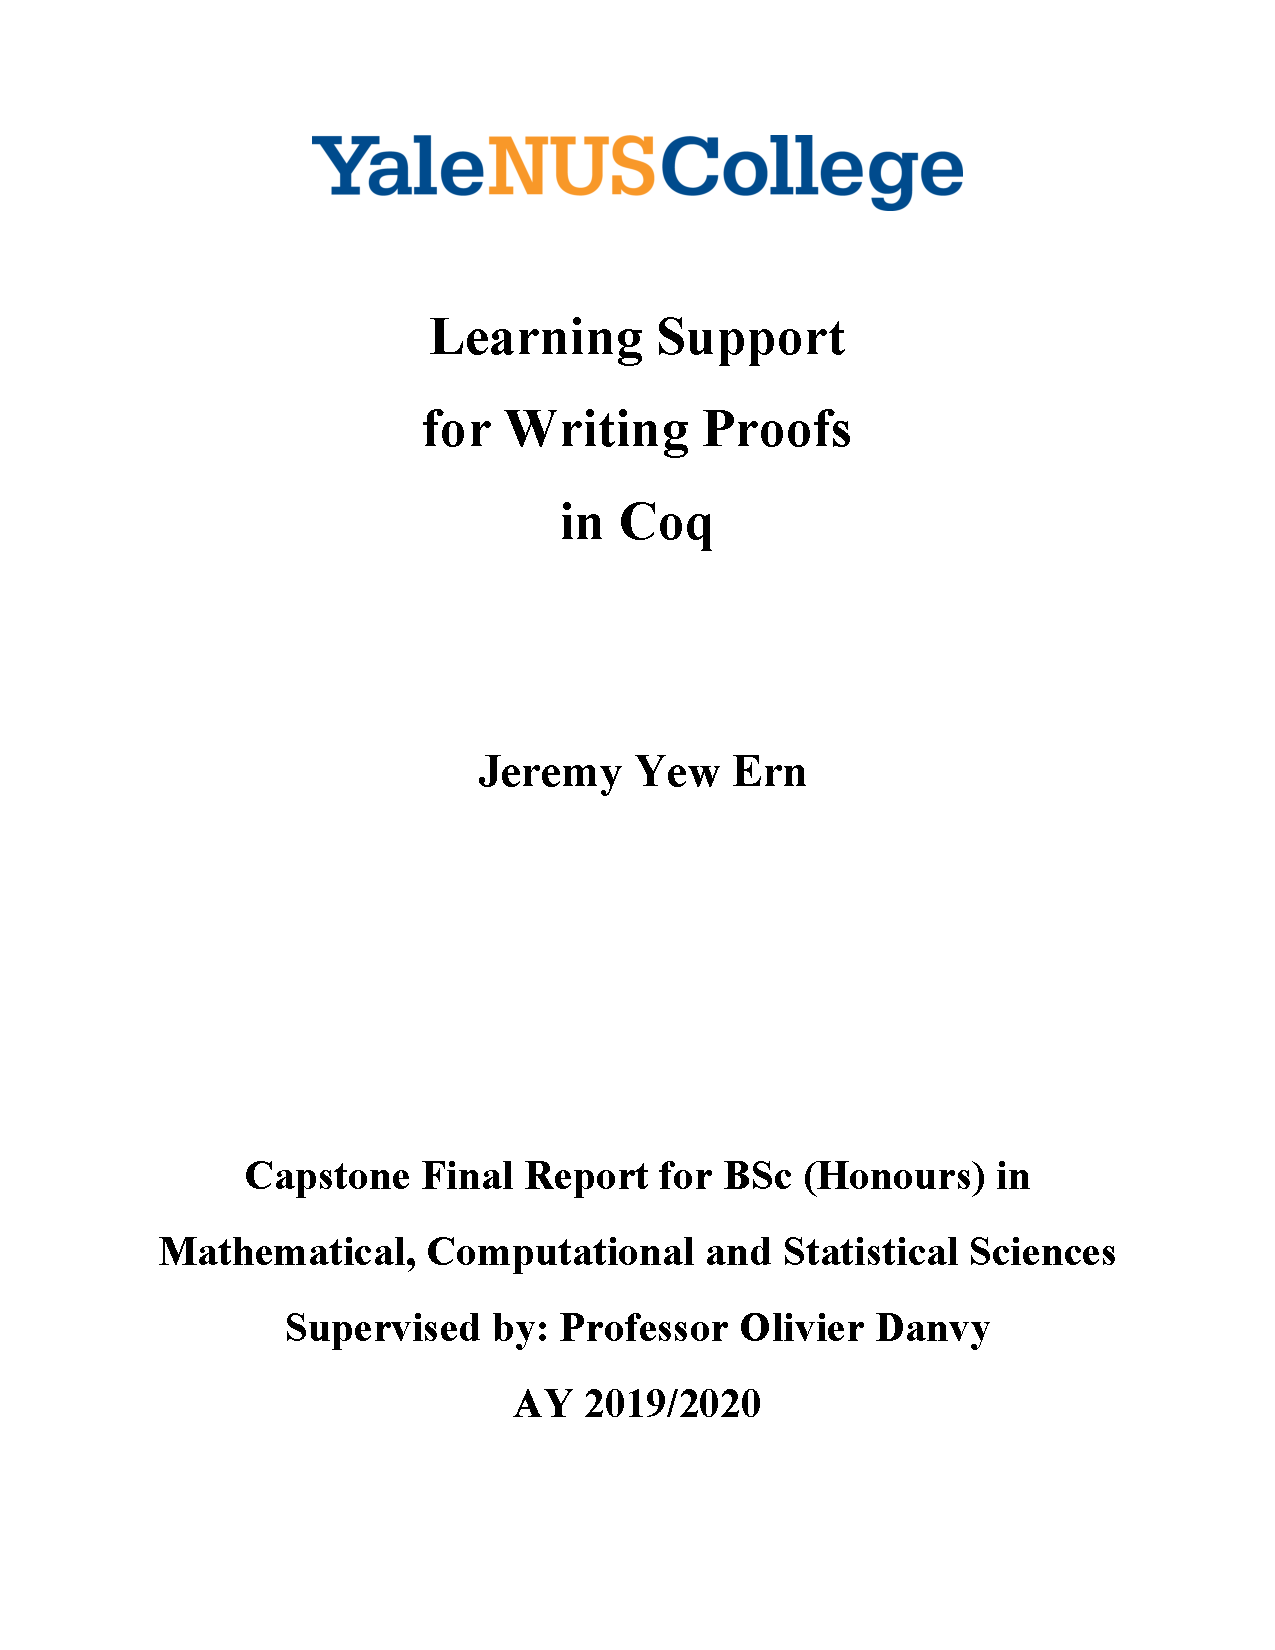
\includepdf[pages=-,pagecommand={},width=\textwidth]{titlepage.pdf}

\end{titlepage}

%----------------------------------------------------------------------------------------
%	DECLARATION & CONSENT
%----------------------------------------------------------------------------------------

% print, sign, and scan the declaration form, then include it here
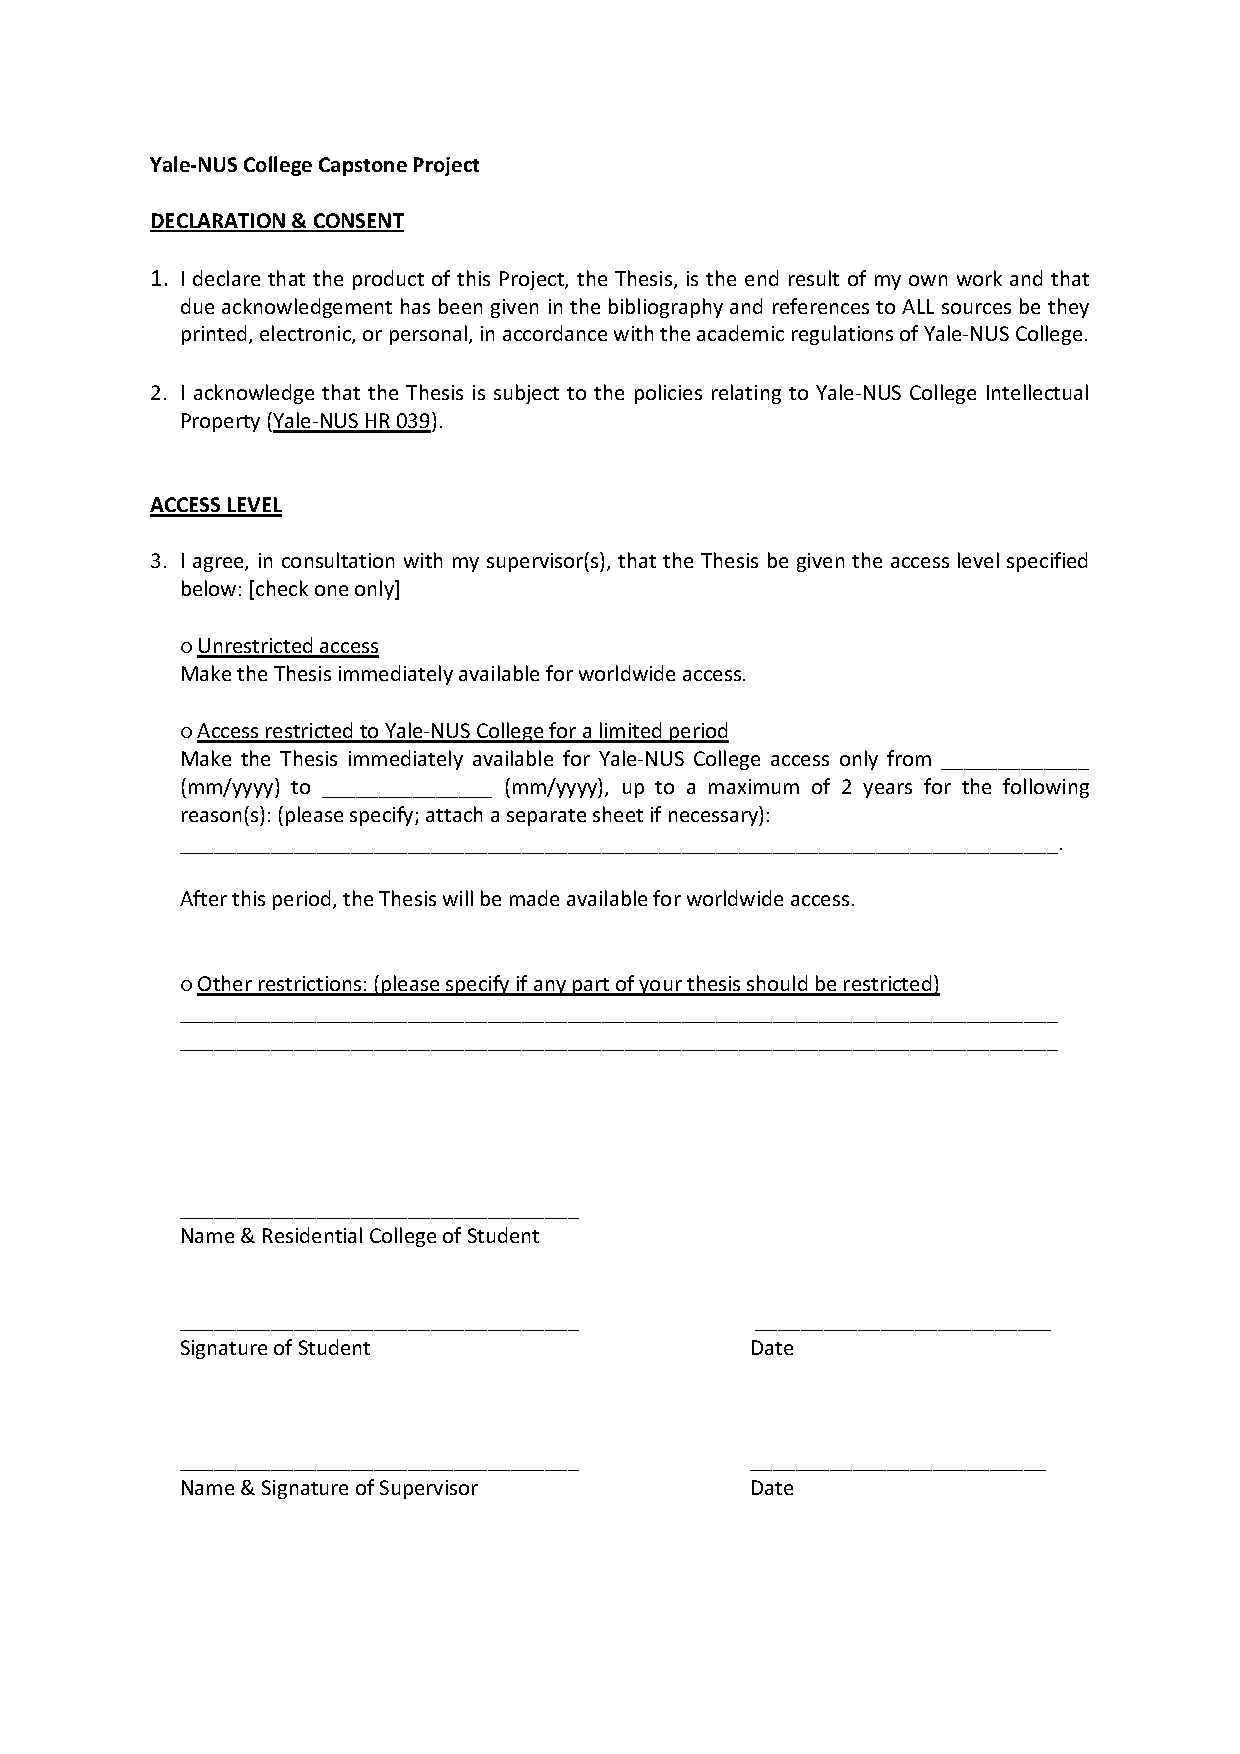
\includepdf[pages=-,pagecommand={},width=\textwidth]{declaration.pdf}

%----------------------------------------------------------------------------------------
%	ACKNOWLEDGEMENTS
%----------------------------------------------------------------------------------------

\begin{acknowledgements}
	\addchaptertocentry{\acknowledgementname} % Add the acknowledgements to the table of contents
	I would like to acknowledge Prof Danvy for his generous and dedicated guidance.
\end{acknowledgements}

%----------------------------------------------------------------------------------------
%	ABSTRACT PAGE
%----------------------------------------------------------------------------------------

\begin{abstract}
	\addchaptertocentry{\abstractname} % Add the abstract to the table of contents
	This project provides learning support for students enrolled in YSC3216: Functional Programming and Proving (FPP), by providing \code{proof-reader}: an Emacs-integrated tool that acts a set of ’safety rails’, guiding students as they build muscle memory for good proving and programming habits. \code{proof-reader} analyzes student submissions and generates corrective suggestions, thus automating intervention on syntax issues, which is usually performed via written feedback by the course instructor. This allows the instructor to focus on substantive rather than superficial feedback. The tool is intended to be used interactively by students, both during proof editing and before submission.
\end{abstract}


%----------------------------------------------------------------------------------------
% CONTRIBUTIONS
%----------------------------------------------------------------------------------------

% \chapter{Claims}
%
% This paper presents the following original contributions:
%
% \begin{enumerate}
% 	\item A hardware device for haptic sensory substitution along with designs for the construction of such a system.
% 	\item Two implementations of sensory substitution using haptic feedback, continuous and delayed feedback-based spatial navigation tasks, each of which include:
% 		\begin{enumerate}
% 			\item a front-end for providing visual input to the user during the training phase with useful readouts to the researcher,
% 			\item a transmission protocol, which maps information from the task at hand (spatial coordinates, velocity information, etc) to time-based sensor actuation signals (20$^{\circ}$ on servo 1, 35$^{\circ}$ on servo 2, etc) in real-time.
% 		\end{enumerate}
% 	\item An evaluation framework for measuring the performance of a sensory substitution system, which provides sample tasks that can be used to standardise and compare performance across the board for future research.
% 	\item A review of existing hardware and software stacks as well as possible avenues for development based on the developed metrics.
% \end{enumerate}
%
% In addition, code for displaying results in real-time, modules for managing servo overload, network latency and other factors were also written by the author.


% %----------------------------------------------------------------------------------------
% %	DECLARATION PAGE
% %----------------------------------------------------------------------------------------
%
% \begin{declaration}
% \addchaptertocentry{\authorshipname} % Add the declaration to the table of contents
%
% \noindent I, \authorname, hereby declare that this Project, the Capstone Report and associated work listed herein, is the end result of my own work and that due acknowledgement has been given in the bibliography and references to ALL sources printed, electronic, or personal, in accordance with the academic regulations of Yale‐NUS College.
% I acknowledge that the Thesis is subject to the policies relating to Yale‐NUS College Intellectual  Property (Yale‐NUS HR 039).
%
%
% % I confirm that:
% %
% % \begin{itemize}
% % \item This work was done wholly or mainly while in candidature for a research degree at this University.
% % \item Where any part of this thesis has previously been submitted for a degree or any other qualification at this University or any other institution, this has been clearly stated.
% % \item Where I have consulted the published work of others, this is always clearly attributed.
% % \item Where I have quoted from the work of others, the source is always given. With the exception of such quotations, this thesis is entirely my own work.
% % \item I have acknowledged all main sources of help.
% % \item Where the thesis is based on work done by myself jointly with others, I have made clear exactly what was done by others and what I have contributed myself.\\
% % \end{itemize}
%
% \noindent Signed:\\
% \rule[0.5em]{25em}{0.5pt} % This prints a line for the signature
%
% \noindent Date:\\
% \rule[0.5em]{25em}{0.5pt} % This prints a line to write the date
% \end{declaration}
%
% \cleardoublepage

%----------------------------------------------------------------------------------------
%	QUOTATION PAGE
%----------------------------------------------------------------------------------------

% \vspace*{0.2\textheight}
%
% \noindent\enquote{\itshape Thanks to my solid academic training, today I can write hundreds of words on virtually any topic without possessing a shred of information, which is how I got a good job in journalism.}\bigbreak
%
% \hfill Dave Barry

%----------------------------------------------------------------------------------------
%	LIST OF CONTENTS/FIGURES/TABLES PAGES
%----------------------------------------------------------------------------------------

\tableofcontents % Prints the main table of contents

% \listoftables % Prints the list of tables
% \label{lst:tabs}

% \listoffigures % Prints the list of figures
% \label{lst:figs}
%----------------------------------------------------------------------------------------
%	ABBREVIATIONS
%----------------------------------------------------------------------------------------

% \begin{abbreviations}{ll} % Include a list of abbreviations (a table of two columns)
%
% \textbf{LAH} & \textbf{L}ist \textbf{A}bbreviations \textbf{H}ere\\
% \textbf{WSF} & \textbf{W}hat (it) \textbf{S}tands \textbf{F}or\\
%
% \end{abbreviations}

%----------------------------------------------------------------------------------------
%	PHYSICAL CONSTANTS/OTHER DEFINITIONS
%----------------------------------------------------------------------------------------

% \begin{constants}{lr@{${}={}$}l} % The list of physical constants is a three column table
%
% % The \SI{}{} command is provided by the siunitx package, see its documentation for instructions on how to use it
%
% Speed of Light & $c_{0}$ & \SI{2.99792458e8}{\meter\per\second} (exact)\\
% %Constant Name & $Symbol$ & $Constant Value$ with units\\
%
% \end{constants}

%----------------------------------------------------------------------------------------
%	SYMBOLS
%----------------------------------------------------------------------------------------

% \begin{symbols}{lll} % Include a list of Symbols (a three column table)
%
% $a$ & distance & \si{\meter} \\
% $P$ & power & \si{\watt} (\si{\joule\per\second}) \\
% %Symbol & Name & Unit \\
%
% \addlinespace % Gap to separate the Roman symbols from the Greek
%
% $\omega$ & angular frequency & \si{\radian} \\
%
% \end{symbols}

%----------------------------------------------------------------------------------------
%	DEDICATION
%----------------------------------------------------------------------------------------


%----------------------------------------------------------------------------------------
%	THESIS CONTENT - CHAPTERS
%----------------------------------------------------------------------------------------

\mainmatter % Begin numeric (1,2,3...) page numbering

\pagestyle{thesis} % Return the page headers back to the "thesis" style

% Include the chapters of the thesis as separate files from the Chapters folder
% Uncomment the lines as you write the chapters

% % Chapter 1

\chapter{Tips} % Main chapter title

\epigraph{``Y a plein de c\^otes \`a Ibiza\\C'est vraiment dur il fait tr\`es chaud.''}{\textit{Zambla}}

\label{chapter1} % For referencing the chapter elsewhere, use \ref{Chapter1}

%----------------------------------------------------------------------------------------
\section{Introduction}
Dear student reading that chapter, greetings!
After doing some research and writing reports for more than 12 years, I realized that LaTeX is the second worst way to write a thesis.
The worst one is Word.
Then you may be wondering, which is the best way to write a report?
Well, actually there is no best way.
Hence you are stuck with LaTeX.

\subsection{Goal of this chaper}
In this chapter, I will demonstrate a few interesting features of LaTeX, and more importantly, provide examples of Figures, Tables, Equations and Code Snippets.
These may be easy to deal with on Word, but here it is another story.
The general idea is to keep these examples, copy-paste them, then modify them to fit your needs.
If you are seeing this content while reading \texttt{main.pdf}, please load the overall LaTeX project in your LaTeX editor, and open the \texttt{chapters/chaper1.tex}.
\\
\\
Done?
Ok let us move on then!
So by now, you should have noticed a few things:
\begin{itemize}
  \item Each sentence of the text is on a distinct line. Yet, sentences are still within the same paragraph.
  \item Backslash is an escape character, used at the beginning of LaTeX commands.
  \item To end a paragraph (or actually insert a newline), we can use the \textbackslash{}\textbackslash{} command.
\end{itemize}
Also now you know how to do a bullet list.

\subsection{Structure of a chapter}
Chapter contain sections (defined with \textbackslash{}section\{Name of your section\}), subsections (\textbackslash{}subsection).

\subsubsection{Because subsubsection that's why!}
Subsubsections are also available (\textbackslash{}subsubsection).

\paragraph{Paragraph}
If you really insist, there are also paragraphes, which may or may not be the same as a subsubsection.
Note that the automatically generated table of contents only goes to two levels of depth within chapters by default.
This can be changed, but you likely do not want to do that.

\subparagraph{Subparagraph}
I was today years old when I discovered the subparagraph. Seriously, do not use it.

\section{Font Formatting Commands}
Similarly to Word, LaTeX provides simple formatting, including \textbf{bold}, \textit{italic}, \underline{underlined} and \texttt{ugly stuff}.
However, no underline or strikethrough by default.
You can also change the size of the text, using {\tiny tiny}, {\small small}, {\large large}, {\huge huge}.
These last commands work within a specific scope.
The scope can be specified using \{ and \}, with the \{ placed before the \textbackslash{}size command.

\subsection{Special characters}
LaTeX uses 10 special characters. Each of these characters has a special meaning.
\begin{enumerate}
  \item Ampersand (\&) is used in tables as a cell delimiter.
  \item Percent sign (\%) is used for commenting a line.
  \item Dollar sign (\$) is used to switch back/from mathematical notation mode.
  \item Hash sign (\#) is used to create macros --- you definitely do not want to go more in depth here.
  \item Underscore (\_ or \textunderscore) is used to indicate a subscript in maths mode, if you use it in text mode ( without using backslash in front to ''escape'' it), your project will not compile anymore. \textbf{You may want to read that twice, and remember it.} It is in a LaTeX template, therefore it must be true.
  \item Curly brackets (\{ and \}) or bracets are used by LaTeX commands, as you likely already noticed.
  \item Tilde (\textasciitilde) can be used to create a non-breaking space (so that both words are on the same line).
  \item Caret/Circumflex/Hat (\textasciicircum) is used to indicate superscript (exponent) in maths mode.
  \item Backslash (\textbackslash) is used in front of every command. You cannot simply escape it to print it, as \textbackslash{}\textbackslash{} create a new line.
\end{enumerate}
If you happen to insert some of these symbols in your text without either escaping (when possible) or using the correct command, your project will likely not compile.
Thus, you may want to be extra careful about that problem.
Note: the underscore issue may also be encountered with bibliography.
So if \texttt{bibtex} displays an error, it may also come from an underscore somewhere in the abstract, DOI or URL field.

\section{Equations}
Here is an equation:
\begin{equation}
\int_0^\infty e^{-x^2} dx
\label{eq:eq1}
\end{equation}

I could also want to have this equation inline, i.e. within the text: $\int_0^\infty e^{-x^2} dx$.
In that case, simply use \textdollar{} (by the way, note that using the dollar sign in your text switches to mathematical notation. To actually print a dollar sign use the \textbackslash{}textdollar command).
The equation above has a label, meaning you can refer to it. The numbering system uses the chapter number (in this case 1), then the equation position within the chapter (1 again).
Example: Equation~\ref{eq:eq1} is an example of an equation in LaTeX{}.
In case you would like to have an equation without numbering it? Easy!
\begin{equation*}
t = a \times log_{2}(\frac{D}{W} + 1) + b
\end{equation*}

The only difference? The \textasteriskcentered{}  symbol in the \textbackslash{}begin\{equation\textbf{\textasteriskcentered}\}.
This also works with Figures and Tables.

\section{Code Snippets}

\begin{lstlisting}
  int main (int argc, char ** argc)
  {
    printf("Hello world!\n");
    return 0;
  }
\end{lstlisting}

This template uses the \texttt{lstlisting} package, which not the best for code snippets.
However, it works without any problem, while other packages may have compatibility issues.
Feel free to try alternative solutions, the best one being \texttt{minted}.

\section{Figures}
Figures are a bit tricky with LaTeX {\tiny(not as much as tables though)}.
Let us see a simple example below:
\begin{figure}[!h]
  \centering
    
\includegraphics[width=0.9\textwidth]{figures/future.png}
  \caption{When a YNC alumni tells you that back in their days, they did not have LaTeX template and would write their report in latin on a papyrus.}
  \label{fig:future}
\end{figure}
You can refer to it: Figure~\ref{fig:future}.
This is possible thanks to the \textbackslash{}label command.
The figure should also be shown on the \hyperref[lst:figs]{List of Figures} page (note this other way of referring to another part of the manuscript!).
A common practice is use the following naming convention:
\begin{itemize}
  \item A prefix, indicating the nature of the object labelled: \texttt{eq} for equations, \texttt{fig} for figures, \texttt{tab} for tables.
  \item A colon.
  \item A unique name (easy to remember) describing your figure. Example: exp1confmatrix would suggest that the figure shows a confusion matrix for your experiment 1.
\end{itemize}

A few other points: The \textbackslash{}caption and \textbackslash{}label can be put either before or after the \textbackslash{}includegraphics command.
When you create a Figure, you need to provide placement information for LaTeX. LaTeX will usually not locate the figures \emph{exactly} where you want them.
The most common specifiers are: \texttt{h} (here), \texttt{b} (bottom of the page) and \texttt{t} (top). The \texttt{!} specifier tries to force LaTeX to put the image exactly at the location you specified (with mixed success though).
For a longer list of specifiers, please refer to: \url{https://en.wikibooks.org/wiki/LaTeX/Floats,_Figures_and_Captions}.

\subsection{Figure Size}
The size of the figure can be determined by the first parameter of the \textbackslash{}includegraphics command.
In this example, we set the size to be $0.9 \times \texttt{textwidth}$, or 90\% of the size of a column.
We could have used an absolute value in cm, e.g. \texttt{width=19cm}.

\subsection{Supported Formats}
Use standard formats, such as PNG, PDF, JPG.
LaTeX also supports other formats, such as EPS.
\textbf{Rule of thumb: use PDF as much as you can, as it uses vector graphics, making it easy to scale the figure to very large format without problems.}

\subsection{Multiple images in one figure}
You can also create complex figures with multiple images.
Here is an example, which uses a $2\times2$ layout.
The overall figure can be referred as Figure~\ref{fig:drake}.
\begin{figure}[!h]
  \begin{subfigure}[t]{.5\textwidth}
    \centering
    
\includegraphics[width=\linewidth]{figures/draketl.png}
    %\caption{We could totally insert a caption here}
    %\label{fig:draketl}
  \end{subfigure}
  \hfill
  \begin{subfigure}[t]{.5\textwidth}
    \centering
    
\includegraphics[width=\linewidth]{figures/draketr.png}
    %\caption{We could totally insert a caption here}
        %\label{fig:draketr}
  \end{subfigure}

  %\medskip
  % the medskip will have white space between both lines
  \begin{subfigure}[t]{.5\textwidth}
    \centering
    
\includegraphics[width=\linewidth]{figures/drakebl}
    %\caption{We could totally insert a caption here}
        %\label{fig:drakebl}
  \end{subfigure}
  \hfill
  \begin{subfigure}[t]{.5\textwidth}
    \centering
    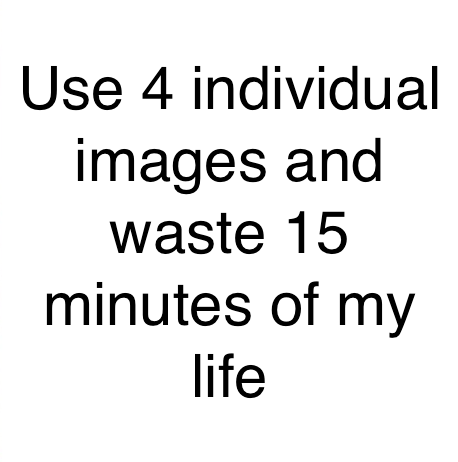
\includegraphics[width=\linewidth]{figures/drakebr}
    %\caption{We could totally insert a caption here}
    %\label{fig:drakebr}
  \end{subfigure}
  \caption{Example of a complex figures on a $2\times2$ layout.}
  \label{fig:drake}
\end{figure}

\section{Tables}
Tables can be a nightmare in LaTeX.
The easiest way to deal with tables in LaTeX is to use some online tools.
My favorite so far: \url{https://www.tablesgenerator.com/}

Here is an example of confusion matrix generated:
\begin{table}[!h]
  \resizebox{\textwidth}{!}{
\begin{tabular}{|c|c|ccccccccc}
\cline{1-2}
Chest (C)                         & -     &                                                                          &                                                                           &                                                                          &                          &                            &                           &                           &                            &                                                                            \\ \cline{1-3}
Chest (ND)  & *     & \multicolumn{1}{c|}{-}                                                   &                                                                           &                                                                          &                          &                            &                           &                           &                            &                                                                            \\ \cline{1-4}
Chest (D)   & *     & \multicolumn{1}{c|}{-}                                                   & \multicolumn{1}{c|}{*}                                                    &                                                                          &                          &                            &                           &                           &                            &                                                                            \\ \cline{1-5}
Ear          & -     & \multicolumn{1}{c|}{-}                                                   & \multicolumn{1}{c|}{-}                                                    & \multicolumn{1}{c|}{}                                                    &                          &                            &                           &                           &                            &                                                                            \\ \cline{1-6}
Thigh       & *     & \multicolumn{1}{c|}{-}                                                   & \multicolumn{1}{c|}{*}                                                    & \multicolumn{1}{c|}{*}                                                   & \multicolumn{1}{c|}{-}   &                            &                           &                           &                            &                                                                            \\ \cline{1-7}
Neck        & -     & \multicolumn{1}{c|}{*}                                                   & \multicolumn{1}{c|}{-}                                                    & \multicolumn{1}{c|}{*}                                                   & \multicolumn{1}{c|}{-}   & \multicolumn{1}{c|}{-}     &                           &                           &                            &                                                                            \\ \cline{1-8}
Palm        & -     & \multicolumn{1}{c|}{}                                                    & \multicolumn{1}{c|}{*}                                                    & \multicolumn{1}{c|}{-}                                                   & \multicolumn{1}{c|}{-}   & \multicolumn{1}{c|}{-}     & \multicolumn{1}{c|}{-}    &                           &                            &                                                                            \\ \cline{1-9}
Thumb       & -     & \multicolumn{1}{c|}{*}                                                   & \multicolumn{1}{c|}{-}                                                    & \multicolumn{1}{c|}{*}                                                   & \multicolumn{1}{c|}{-}   & \multicolumn{1}{c|}{-}     & \multicolumn{1}{c|}{*}    & \multicolumn{1}{c|}{*}    &                            &                                                                            \\ \cline{1-10}
Inner Wrist & *     & \multicolumn{1}{c|}{-}                                                   & \multicolumn{1}{c|}{-}                                                    & \multicolumn{1}{c|}{-}                                                   & \multicolumn{1}{c|}{*}   & \multicolumn{1}{c|}{*}     & \multicolumn{1}{c|}{*}    & \multicolumn{1}{c|}{-}    & \multicolumn{1}{c|}{*}     &                                                                            \\ \hline
Outer Wrist & -     & \multicolumn{1}{c|}{*}                                                   & \multicolumn{1}{c|}{-}                                                    & \multicolumn{1}{c|}{*}                                                   & \multicolumn{1}{c|}{-}   & \multicolumn{1}{c|}{-}     & \multicolumn{1}{c|}{-}    & \multicolumn{1}{c|}{*}    & \multicolumn{1}{c|}{-}     & \multicolumn{1}{c|}{-}                                                     \\ \hline
  & Belly & \multicolumn{1}{c|}{\begin{tabular}[c]{@{}c@{}}Chest\\ (C)\end{tabular}} & \multicolumn{1}{c|}{\begin{tabular}[c]{@{}c@{}}Chest\\ (ND)\end{tabular}} & \multicolumn{1}{c|}{\begin{tabular}[c]{@{}c@{}}Chest\\ (D)\end{tabular}} & \multicolumn{1}{c|}{Ear} & \multicolumn{1}{c|}{Thigh} & \multicolumn{1}{c|}{Neck} & \multicolumn{1}{c|}{Palm} & \multicolumn{1}{c|}{Thumb} & \multicolumn{1}{c|}{\begin{tabular}[c]{@{}c@{}}Inner\\ Wrist\end{tabular}} \\ \hline
\end{tabular}
}
\caption{Post-hoc comparisons between body parts. - shows no significant difference ($p>.05$), \textasteriskcentered{} shows differences ($p<.05$).}
\label{tab:posthoc}
\end{table}

Note that a table is actually a container for another type of LaTeX object, \emph{tabular}.
Tables come with captions and label, allowing us to refer to Table~\ref{tab:posthoc}.
Another interesting point is that the \textbackslash{}begin\{tabular\} command uses characters.
These characters specify how the text should be centered within each cell: \texttt{c} means centered, \texttt{l} means left and \texttt{r} means right.
Finally, my original table was too large to fit a page, so I used the \textbackslash{}resizebox\{\textbackslash{}textwidth\}\{!\}\{ command.
This command needs a closing \} after the \textbackslash{}end\{tabular\} command.
This table is also now shown in the \hyperref[lst:tabs]{List of Tables} page.
\\
\textbf{Anyway, for Tables, using the LaTeX Table Generator is a great option.}

\section{Bibliography}
LaTeX{} is really convenient to deal with bibliography.
All your references should be in a \texttt{\textasteriskcentered.bib} file.
Each reference has a unique key, that you will use to refer to that publication.

You can simply cite nearly anything using the \textbackslash{}cite command.
You can cite conference papers, e.g. ``WatchIt (\cite{Perrault2013}) is an interactive wristband for smart watches.'' or journal articles, e.g. ``Lopez et al. (\cite{Lopez2017}) ran a public consultation in Mexico''.
In the first example, the key in the bib file is Perrault2013, see\\

\includegraphics{figures/bibtexkey}

\subsection{How to get Bibtex References?}
The easiest way to find the Bibtex snippet you need for a given reference is to use Google Scholar~(\cite{Scholar}).
On the main page, type the name of the paper you are looking for.
\\

In the results page, locate the paper:
\begin{figure}[!h]
  \centering
    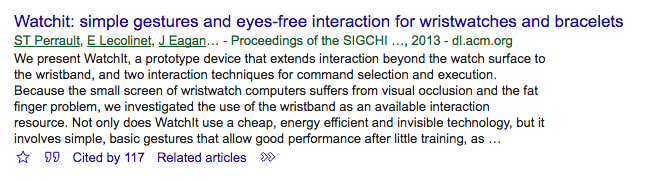
\includegraphics[width=0.9\textwidth]{figures/scholarrefexample.png}
  \caption{Example of result on Scholar}
  \label{fig:scholarref}
\end{figure}

On the last line of the result (shown in Figure~\ref{fig:scholarref}), there is a \textbf{''} symbol.
Clicking on it will display a pop-up.
\begin{figure}[!h]
  \centering
    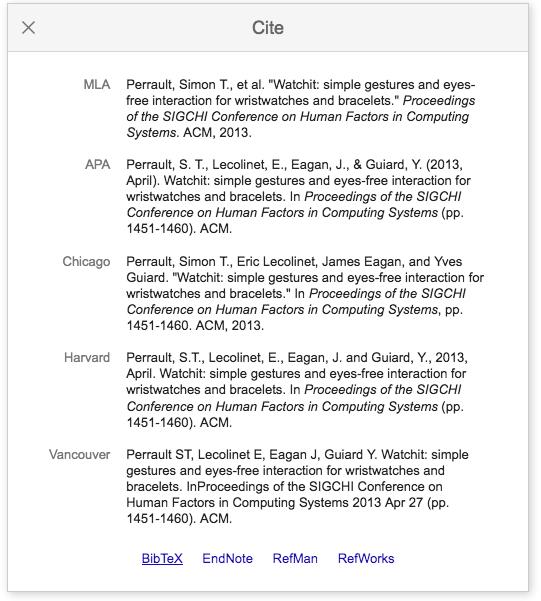
\includegraphics[width=0.7\textwidth]{figures/scholarpopup.png}
  \caption{Pop-up window with the possible citations}
  \label{fig:scholarpopup}
\end{figure}
\\

At the bottom (see Figure~\ref{fig:scholarpopup}), you will notice a ``Bibtex'' link. Click on it.
Scholar will then display a small block of text starting with @ symbol.
Copy and paste this snippet in your \texttt{biblio.bib} and you are done.
You may eventually want to check the citation key to something shorter.
\\

\textbf{You may get unexpected compilation errors with some references. The most common case is that the bibtex entry contains a DOI field, which in turn contains an underscore (\_).}
If that is the case, simply remove the DOI field (not a great practice but a good workaround).

\section{End of the Tips}
We are now done with the tips.
The next chapter contains more explanations and specificites of LaTeX{} and the template used here.
Good luck with your capstone report.

% \chapter{Chapter Title Here} % Main chapter title


\label{chapter2} % For referencing the chapter elsewhere, use \ref{Chapter1}

\epigraph{``Seriously, who puts stupid quotes at the beginning of a chapter? A quote alone will not give me more points on the report anyway.''}{\textit{You, dawn of the 3rd day}}

%----------------------------------------------------------------------------------------
We can reference other chapters, for example, here we refer to Chapter~\ref{chapter1}.

%----------------------------------------------------------------------------------------

% Define some commands to keep the formatting separated from the content
\newcommand{\keyword}[1]{\textbf{#1}}
\newcommand{\tabhead}[1]{\textbf{#1}}
\newcommand{\code}[1]{\texttt{#1}}
\newcommand{\file}[1]{\texttt{\bfseries#1}}
\newcommand{\option}[1]{\texttt{\itshape#1}}

%----------------------------------------------------------------------------------------

\section{Welcome and Thank You}
Welcome to this \LaTeX{} Thesis Template, a beautiful and easy to use template for writing a thesis using the \LaTeX{} typesetting system.

If you are writing a thesis (or will be in the future) and its subject is technical or mathematical (though it doesn't have to be), then creating it in \LaTeX{} is highly recommended as a way to make sure you can just get down to the essential writing without having to worry over formatting or wasting time arguing with your word processor.

\LaTeX{} is easily able to professionally typeset documents that run to hundreds or thousands of pages long. With simple mark-up commands, it automatically sets out the table of contents, margins, page headers and footers and keeps the formatting consistent and beautiful. One of its main strengths is the way it can easily typeset mathematics, even \emph{heavy} mathematics. Even if those equations are the most horribly twisted and most difficult mathematical problems that can only be solved on a super-computer, you can at least count on \LaTeX{} to make them look stunning.

%----------------------------------------------------------------------------------------

\section{Learning \LaTeX{}}

\LaTeX{} is not a \textsc{wysiwyg} (What You See is What You Get) program, unlike word processors such as Microsoft Word or Apple's Pages. Instead, a document written for \LaTeX{} is actually a simple, plain text file that contains \emph{no formatting}. You tell \LaTeX{} how you want the formatting in the finished document by writing in simple commands amongst the text, for example, if I want to use \emph{italic text for emphasis}, I write the \verb|\emph{text}| command and put the text I want in italics in between the curly braces. This means that \LaTeX{} is a \enquote{mark-up} language, very much like HTML.

\subsection{A (not so short) Introduction to \LaTeX{}}

If you are new to \LaTeX{}, there is a very good eBook -- freely available online as a PDF file -- called, \enquote{The Not So Short Introduction to \LaTeX{}}. The book's title is typically shortened to just \emph{lshort}. You can download the latest version (as it is occasionally updated) from here:
\url{http://www.ctan.org/tex-archive/info/lshort/english/lshort.pdf}

It is also available in several other languages. Find yours from the list on this page: \url{http://www.ctan.org/tex-archive/info/lshort/}

It is recommended to take a little time out to learn how to use \LaTeX{} by creating several, small `test' documents, or having a close look at several templates on:\\
\url{http://www.LaTeXTemplates.com}\\
Making the effort now means you're not stuck learning the system when what you \emph{really} need to be doing is writing your thesis.

\subsection{A Short Math Guide for \LaTeX{}}

If you are writing a technical or mathematical thesis, then you may want to read the document by the AMS (American Mathematical Society) called, \enquote{A Short Math Guide for \LaTeX{}}. It can be found online here:
\url{http://www.ams.org/tex/amslatex.html}
under the \enquote{Additional Documentation} section towards the bottom of the page.

\subsection{Common \LaTeX{} Math Symbols}
There are a multitude of mathematical symbols available for \LaTeX{} and it would take a great effort to learn the commands for them all. The most common ones you are likely to use are shown on this page:
\url{http://www.sunilpatel.co.uk/latex-type/latex-math-symbols/}

You can use this page as a reference or crib sheet, the symbols are rendered as large, high quality images so you can quickly find the \LaTeX{} command for the symbol you need.

\subsection{\LaTeX{} on a Mac}

The \LaTeX{} distribution is available for many systems including Windows, Linux and Mac OS X. The package for OS X is called MacTeX and it contains all the applications you need -- bundled together and pre-customized -- for a fully working \LaTeX{} environment and work flow.

MacTeX includes a custom dedicated \LaTeX{} editor called TeXShop for writing your `\file{.tex}' files and BibDesk: a program to manage your references and create your bibliography section just as easily as managing songs and creating playlists in iTunes.

%----------------------------------------------------------------------------------------

\section{Getting Started with this Template}

If you are familiar with \LaTeX{}, then you should explore the directory structure of the template and then proceed to place your own information into the \emph{THESIS INFORMATION} block of the \file{main.tex} file. You can then modify the rest of this file to your unique specifications based on your degree/university. Section \ref{FillingFile} on page \pageref{FillingFile} will help you do this. Make sure you also read section \ref{ThesisConventions} about thesis conventions to get the most out of this template.

If you are new to \LaTeX{} it is recommended that you carry on reading through the rest of the information in this document.

Before you begin using this template you should ensure that its style complies with the thesis style guidelines imposed by your institution. In most cases this template style and layout will be suitable. If it is not, it may only require a small change to bring the template in line with your institution's recommendations. These modifications will need to be done on the \file{MastersDoctoralThesis.cls} file.

\subsection{About this Template}

This \LaTeX{} Thesis Template is originally based and created around a \LaTeX{} style file created by Steve R.\ Gunn from the University of Southampton (UK), department of Electronics and Computer Science. You can find his original thesis style file at his site, here:
\url{http://www.ecs.soton.ac.uk/~srg/softwaretools/document/templates/}

Steve's \file{ecsthesis.cls} was then taken by Sunil Patel who modified it by creating a skeleton framework and folder structure to place the thesis files in. The resulting template can be found on Sunil's site here:
\url{http://www.sunilpatel.co.uk/thesis-template}

Sunil's template was made available through \url{http://www.LaTeXTemplates.com} where it was modified many times based on user requests and questions. Version 2.0 and onwards of this template represents a major modification to Sunil's template and is, in fact, hardly recognisable. The work to make version 2.0 possible was carried out by \href{mailto:vel@latextemplates.com}{Vel} and Johannes Böttcher.

%----------------------------------------------------------------------------------------

\section{What this Template Includes}

\subsection{Folders}

This template comes as a single zip file that expands out to several files and folders. The folder names are mostly self-explanatory:

\keyword{Appendices} -- this is the folder where you put the appendices. Each appendix should go into its own separate \file{.tex} file. An example and template are included in the directory.

\keyword{Chapters} -- this is the folder where you put the thesis chapters. A thesis usually has about six chapters, though there is no hard rule on this. Each chapter should go in its own separate \file{.tex} file and they can be split as:
\begin{itemize}
\item Chapter 1: Introduction to the thesis topic
\item Chapter 2: Background information and theory
\item Chapter 3: (Laboratory) experimental setup
\item Chapter 4: Details of experiment 1
\item Chapter 5: Details of experiment 2
\item Chapter 6: Discussion of the experimental results
\item Chapter 7: Conclusion and future directions
\end{itemize}
This chapter layout is specialised for the experimental sciences, your discipline may be different.

\keyword{Figures} -- this folder contains all figures for the thesis. These are the final images that will go into the thesis document.

\subsection{Files}

Included are also several files, most of them are plain text and you can see their contents in a text editor. After initial compilation, you will see that more auxiliary files are created by \LaTeX{} or BibTeX and which you don't need to delete or worry about:

\keyword{example.bib} -- this is an important file that contains all the bibliographic information and references that you will be citing in the thesis for use with BibTeX. You can write it manually, but there are reference manager programs available that will create and manage it for you. Bibliographies in \LaTeX{} are a large subject and you may need to read about BibTeX before starting with this. Many modern reference managers will allow you to export your references in BibTeX format which greatly eases the amount of work you have to do.

\keyword{MastersDoctoralThesis.cls} -- this is an important file. It is the class file that tells \LaTeX{} how to format the thesis.

\keyword{main.pdf} -- this is your beautifully typeset thesis (in the PDF file format) created by \LaTeX{}. It is supplied in the PDF with the template and after you compile the template you should get an identical version.

\keyword{main.tex} -- this is an important file. This is the file that you tell \LaTeX{} to compile to produce your thesis as a PDF file. It contains the framework and constructs that tell \LaTeX{} how to layout the thesis. It is heavily commented so you can read exactly what each line of code does and why it is there. After you put your own information into the \emph{THESIS INFORMATION} block -- you have now started your thesis!

Files that are \emph{not} included, but are created by \LaTeX{} as auxiliary files include:

\keyword{main.aux} -- this is an auxiliary file generated by \LaTeX{}, if it is deleted \LaTeX{} simply regenerates it when you run the main \file{.tex} file.

\keyword{main.bbl} -- this is an auxiliary file generated by BibTeX, if it is deleted, BibTeX simply regenerates it when you run the \file{main.aux} file. Whereas the \file{.bib} file contains all the references you have, this \file{.bbl} file contains the references you have actually cited in the thesis and is used to build the bibliography section of the thesis.

\keyword{main.blg} -- this is an auxiliary file generated by BibTeX, if it is deleted BibTeX simply regenerates it when you run the main \file{.aux} file.

\keyword{main.lof} -- this is an auxiliary file generated by \LaTeX{}, if it is deleted \LaTeX{} simply regenerates it when you run the main \file{.tex} file. It tells \LaTeX{} how to build the \emph{List of Figures} section.

\keyword{main.log} -- this is an auxiliary file generated by \LaTeX{}, if it is deleted \LaTeX{} simply regenerates it when you run the main \file{.tex} file. It contains messages from \LaTeX{}, if you receive errors and warnings from \LaTeX{}, they will be in this \file{.log} file.

\keyword{main.lot} -- this is an auxiliary file generated by \LaTeX{}, if it is deleted \LaTeX{} simply regenerates it when you run the main \file{.tex} file. It tells \LaTeX{} how to build the \emph{List of Tables} section.

\keyword{main.out} -- this is an auxiliary file generated by \LaTeX{}, if it is deleted \LaTeX{} simply regenerates it when you run the main \file{.tex} file.

So from this long list, only the files with the \file{.bib}, \file{.cls} and \file{.tex} extensions are the most important ones. The other auxiliary files can be ignored or deleted as \LaTeX{} and BibTeX will regenerate them.

%----------------------------------------------------------------------------------------

\section{Filling in Your Information in the \file{main.tex} File}\label{FillingFile}

You will need to personalise the thesis template and make it your own by filling in your own information. This is done by editing the \file{main.tex} file in a text editor or your favourite LaTeX environment.

Open the file and scroll down to the third large block titled \emph{THESIS INFORMATION} where you can see the entries for \emph{University Name}, \emph{Department Name}, etc \ldots

Fill out the information about yourself, your group and institution. You can also insert web links, if you do, make sure you use the full URL, including the \code{http://} for this. If you don't want these to be linked, simply remove the \verb|\href{url}{name}| and only leave the name.

When you have done this, save the file and recompile \code{main.tex}. All the information you filled in should now be in the PDF, complete with web links. You can now begin your thesis proper!

%----------------------------------------------------------------------------------------

\section{The \code{main.tex} File Explained}

The \file{main.tex} file contains the structure of the thesis. There are plenty of written comments that explain what pages, sections and formatting the \LaTeX{} code is creating. Each major document element is divided into commented blocks with titles in all capitals to make it obvious what the following bit of code is doing. Initially there seems to be a lot of \LaTeX{} code, but this is all formatting, and it has all been taken care of so you don't have to do it.

Begin by checking that your information on the title page is correct. For the thesis declaration, your institution may insist on something different than the text given. If this is the case, just replace what you see with what is required in the \emph{DECLARATION PAGE} block.

Then comes a page which contains a funny quote. You can put your own, or quote your favourite scientist, author, person, and so on. Make sure to put the name of the person who you took the quote from.

Following this is the abstract page which summarises your work in a condensed way and can almost be used as a standalone document to describe what you have done. The text you write will cause the heading to move up so don't worry about running out of space.

Next come the acknowledgements. On this page, write about all the people who you wish to thank (not forgetting parents, partners and your advisor/supervisor).

The contents pages, list of figures and tables are all taken care of for you and do not need to be manually created or edited. The next set of pages are more likely to be optional and can be deleted since they are for a more technical thesis: insert a list of abbreviations you have used in the thesis, then a list of the physical constants and numbers you refer to and finally, a list of mathematical symbols used in any formulae. Making the effort to fill these tables means the reader has a one-stop place to refer to instead of searching the internet and references to try and find out what you meant by certain abbreviations or symbols.

The list of symbols is split into the Roman and Greek alphabets. Whereas the abbreviations and symbols ought to be listed in alphabetical order (and this is \emph{not} done automatically for you) the list of physical constants should be grouped into similar themes.

The next page contains a one line dedication. Who will you dedicate your thesis to?

Finally, there is the block where the chapters are included. Uncomment the lines (delete the \code{\%} character) as you write the chapters. Each chapter should be written in its own file and put into the \emph{Chapters} folder and named \file{Chapter1}, \file{Chapter2}, etc\ldots Similarly for the appendices, uncomment the lines as you need them. Each appendix should go into its own file and placed in the \emph{Appendices} folder.

After the preamble, chapters and appendices finally comes the bibliography. The bibliography style (called \option{authoryear}) is used for the bibliography and is a fully featured style that will even include links to where the referenced paper can be found online. Do not underestimate how grateful your reader will be to find that a reference to a paper is just a click away. Of course, this relies on you putting the URL information into the BibTeX file in the first place.

%----------------------------------------------------------------------------------------

\section{Thesis Features and Conventions}\label{ThesisConventions}

To get the best out of this template, there are a few conventions that you may want to follow.

One of the most important (and most difficult) things to keep track of in such a long document as a thesis is consistency. Using certain conventions and ways of doing things (such as using a Todo list) makes the job easier. Of course, all of these are optional and you can adopt your own method.

\subsection{Printing Format}

This thesis template is designed for double sided printing (i.e. content on the front and back of pages) as most theses are printed and bound this way. Switching to one sided printing is as simple as uncommenting the \option{oneside} option of the \code{documentclass} command at the top of the \file{main.tex} file. You may then wish to adjust the margins to suit specifications from your institution.

The headers for the pages contain the page number on the outer side (so it is easy to flick through to the page you want) and the chapter name on the inner side.

The text is set to 11 point by default with single line spacing, again, you can tune the text size and spacing should you want or need to using the options at the very start of \file{main.tex}. The spacing can be changed similarly by replacing the \option{singlespacing} with \option{onehalfspacing} or \option{doublespacing}.

\subsection{Using US Letter Paper}

The paper size used in the template is A4, which is the standard size in Europe. If you are using this thesis template elsewhere and particularly in the United States, then you may have to change the A4 paper size to the US Letter size. This can be done in the margins settings section in \file{main.tex}.

Due to the differences in the paper size, the resulting margins may be different to what you like or require (as it is common for institutions to dictate certain margin sizes). If this is the case, then the margin sizes can be tweaked by modifying the values in the same block as where you set the paper size. Now your document should be set up for US Letter paper size with suitable margins.

\subsection{References}

The \code{biblatex} package is used to format the bibliography and inserts references such as this one \parencite{Reference1}. The options used in the \file{main.tex} file mean that the in-text citations of references are formatted with the author(s) listed with the date of the publication. Multiple references are separated by semicolons (e.g. \parencite{Reference2, Reference1}) and references with more than three authors only show the first author with \emph{et al.} indicating there are more authors (e.g. \parencite{Reference3}). This is done automatically for you. To see how you use references, have a look at the \file{Chapter1.tex} source file. Many reference managers allow you to simply drag the reference into the document as you type.

Scientific references should come \emph{before} the punctuation mark if there is one (such as a comma or period). The same goes for footnotes\footnote{Such as this footnote, here down at the bottom of the page.}. You can change this but the most important thing is to keep the convention consistent throughout the thesis. Footnotes themselves should be full, descriptive sentences (beginning with a capital letter and ending with a full stop). The APA6 states: \enquote{Footnote numbers should be superscripted, [...], following any punctuation mark except a dash.} The Chicago manual of style states: \enquote{A note number should be placed at the end of a sentence or clause. The number follows any punctuation mark except the dash, which it precedes. It follows a closing parenthesis.}

The bibliography is typeset with references listed in alphabetical order by the first author's last name. This is similar to the APA referencing style. To see how \LaTeX{} typesets the bibliography, have a look at the very end of this document (or just click on the reference number links in in-text citations).

\subsubsection{A Note on bibtex}

The bibtex backend used in the template by default does not correctly handle unicode character encoding (i.e. "international" characters). You may see a warning about this in the compilation log and, if your references contain unicode characters, they may not show up correctly or at all. The solution to this is to use the biber backend instead of the outdated bibtex backend. This is done by finding this in \file{main.tex}: \option{backend=bibtex} and changing it to \option{backend=biber}. You will then need to delete all auxiliary BibTeX files and navigate to the template directory in your terminal (command prompt). Once there, simply type \code{biber main} and biber will compile your bibliography. You can then compile \file{main.tex} as normal and your bibliography will be updated. An alternative is to set up your LaTeX editor to compile with biber instead of bibtex, see \href{http://tex.stackexchange.com/questions/154751/biblatex-with-biber-configuring-my-editor-to-avoid-undefined-citations/}{here} for how to do this for various editors.

\subsection{Tables}

Tables are an important way of displaying your results, below is an example table which was generated with this code:

{\small
\begin{verbatim}
\begin{table}
\caption{The effects of treatments X and Y on the four groups studied.}
\label{tab:treatments}
\centering
\begin{tabular}{l l l}
\toprule
\tabhead{Groups} & \tabhead{Treatment X} & \tabhead{Treatment Y} \\
\midrule
1 & 0.2 & 0.8\\
2 & 0.17 & 0.7\\
3 & 0.24 & 0.75\\
4 & 0.68 & 0.3\\
\bottomrule\\
\end{tabular}
\end{table}
\end{verbatim}
}

\begin{table}
\caption{The effects of treatments X and Y on the four groups studied.}
\label{tab:treatments}
\centering
\begin{tabular}{l l l}
\toprule
\tabhead{Groups} & \tabhead{Treatment X} & \tabhead{Treatment Y} \\
\midrule
1 & 0.2 & 0.8\\
2 & 0.17 & 0.7\\
3 & 0.24 & 0.75\\
4 & 0.68 & 0.3\\
\bottomrule\\
\end{tabular}
\end{table}

You can reference tables with \verb|\ref{<label>}| where the label is defined within the table environment. See \file{Chapter1.tex} for an example of the label and citation (e.g. Table~\ref{tab:treatments}).

\subsection{Figures}

There will hopefully be many figures in your thesis (that should be placed in the \emph{Figures} folder). The way to insert figures into your thesis is to use a code template like this:
\begin{verbatim}
\begin{figure}
\centering
\includegraphics{Figures/Electron}
\decoRule
\caption[An Electron]{An electron (artist's impression).}
\label{fig:Electron}
\end{figure}
\end{verbatim}
Also look in the source file. Putting this code into the source file produces the picture of the electron that you can see in the figure below.

\begin{figure}[th]
\centering

\includegraphics{figures/electron}
\decoRule
\caption[An Electron]{An electron (artist's impression).}
\label{fig:Electron}
\end{figure}

Sometimes figures don't always appear where you write them in the source. The placement depends on how much space there is on the page for the figure. Sometimes there is not enough room to fit a figure directly where it should go (in relation to the text) and so \LaTeX{} puts it at the top of the next page. Positioning figures is the job of \LaTeX{} and so you should only worry about making them look good!

Figures usually should have captions just in case you need to refer to them (such as in Figure~\ref{fig:Electron}). The \verb|\caption| command contains two parts, the first part, inside the square brackets is the title that will appear in the \emph{List of Figures}, and so should be short. The second part in the curly brackets should contain the longer and more descriptive caption text.

The \verb|\decoRule| command is optional and simply puts an aesthetic horizontal line below the image. If you do this for one image, do it for all of them.

\LaTeX{} is capable of using images in pdf, jpg and png format.

\subsection{Typesetting mathematics}

If your thesis is going to contain heavy mathematical content, be sure that \LaTeX{} will make it look beautiful, even though it won't be able to solve the equations for you.

The \enquote{Not So Short Introduction to \LaTeX} (available on \href{http://www.ctan.org/tex-archive/info/lshort/english/lshort.pdf}{CTAN}) should tell you everything you need to know for most cases of typesetting mathematics. If you need more information, a much more thorough mathematical guide is available from the AMS called, \enquote{A Short Math Guide to \LaTeX} and can be downloaded from:
\url{ftp://ftp.ams.org/pub/tex/doc/amsmath/short-math-guide.pdf}

There are many different \LaTeX{} symbols to remember, luckily you can find the most common symbols in \href{http://ctan.org/pkg/comprehensive}{The Comprehensive \LaTeX~Symbol List}.

You can write an equation, which is automatically given an equation number by \LaTeX{} like this:
\begin{verbatim}
\begin{equation}
E = mc^{2}
\label{eqn:Einstein}
\end{equation}
\end{verbatim}

This will produce Einstein's famous energy-matter equivalence equation:
\begin{equation}
E = mc^{2}
\label{eqn:Einstein}
\end{equation}

All equations you write (which are not in the middle of paragraph text) are automatically given equation numbers by \LaTeX{}. If you don't want a particular equation numbered, use the unnumbered form:
\begin{verbatim}
\[ a^{2}=4 \]
\end{verbatim}

%----------------------------------------------------------------------------------------

\section{Sectioning and Subsectioning}

You should break your thesis up into nice, bite-sized sections and subsections. \LaTeX{} automatically builds a table of Contents by looking at all the \verb|\chapter{}|, \verb|\section{}|  and \verb|\subsection{}| commands you write in the source.

The Table of Contents should only list the sections to three (3) levels. A \verb|chapter{}| is level zero (0). A \verb|\section{}| is level one (1) and so a \verb|\subsection{}| is level two (2). In your thesis it is likely that you will even use a \verb|subsubsection{}|, which is level three (3). The depth to which the Table of Contents is formatted is set within \file{MastersDoctoralThesis.cls}. If you need this changed, you can do it in \file{main.tex}.

%----------------------------------------------------------------------------------------

\section{In Closing}

You have reached the end of this mini-guide. You can now rename or overwrite this pdf file and begin writing your own \file{Chapter1.tex} and the rest of your thesis. The easy work of setting up the structure and framework has been taken care of for you. It's now your job to fill it out!

Good luck and have lots of fun!

\begin{flushright}
Guide written by ---\\
Sunil Patel: \href{http://www.sunilpatel.co.uk}{www.sunilpatel.co.uk}\\
Vel: \href{http://www.LaTeXTemplates.com}{LaTeXTemplates.com}
\end{flushright}

% Chapter Template

\chapter{Context} % Main chapter title

\label{context} % Change X to a consecutive number; for referencing this chapter elsewhere, use \ref{ChapterX}

%----------------------------------------------------------------------------------------
%	SECTION 1
%----------------------------------------------------------------------------------------

\section{Introduction}
The goal of this project is to provide learning support for students enrolled in YSC3216: Functional Programming and Proving (FPP), by providing a tool that generates corrective suggestions for syntax issues, to be used by students to check their code.

FPP is a course in Yale-NUS College under the Mathematical, Computational and Statistical Sciences major, most recently offered in AY19/20 Semester 1 and taught by Professor Olivier Danvy. FPP introduces students to the Coq proof assistant, which is a system for writing and verifying formal proofs. Throughout the course, students learn that precision and orderliness in their code both reflects and encourages clarity of thought. Therefore, one of the primary learning goals for the first half of the course is to build muscle memory for basic proof techniques and programming habits.

To this end, I implement a program called the \code{proof-reader} that acts a set of ’safety rails’ to guide students towards good proving and programming habits via automated intervention on syntax issues. In particular, this tool will help enforce prescribed techniques: using only tactics introduced in the course, and applying tactics explicitly. Since these issues are often highlighted in written feedback from the instructor, the tool also supports students' learning by greatly reducing the feedback cycle and allowing the instructor to focus on substantive rather than superficial feedback.

The program relies on a grammar specification of a subset of Coq as an input to the tool, which the instructor may modify as the course evolves. The program's interface is a simple Emacs command, and is intended to be used interactively by students, both during proof editing and before submission.

\section{Functional programming (FP)}
Functional programming is a programming paradigm that models programs as mathematical functions. Students taking FPP are expected to have completed the Introduction to Computer Science module, which will have trained them in functional programming (amongst other concepts) using the language OCaml. Coq has a language of programs that is very similar to OCaml, and is in fact written in OCaml.

\subsection{Proving}
In mathematics, a proposition is a statement that either holds or does not hold; a proposition is also sometimes called a theorem or lemma. Proofs may be defined as a logical argument about whether a proposition holds. Proofs use logical rules to demonstrate that what we know or assume to be true – an axiom – implies the truth of something that we do not know - a proposition.

Propositions often contain equations, which are statements asserting the equality of two expressions containing variables. When writing proofs (including proofs in Coq), we exercise equational reasoning: we apply axioms to equations in order to incrementally transform them into something that is clearly true.

\subsection{The Coq proof assistant}
Many proofs in mathematics or computer science are natural language proofs - that is, they are written in a natural language, like English. Since natural languages are often ambiguous, natural language proofs are susceptible to misinterpretation or misconception.

On the other hand, just as there programming languages that express a set of instructions to be executed by a computer, there are also domain-specific languages for writing formal proofs that can be automatically, or mechanically, verified by a computer. Coq allows us to write formal, verifiable proofs in a structured logical language called Gallina, and will also automatically verify that our proofs are syntactically correct as well as type-correct. See \cite{coq-homepage}.

\subsection{YSC3236 Functional Programming and Proving (FPP)}
FPP is taken not only by Yale-NUS students, but also PhD and post-doctoral students from the National University of Singapore (NUS) School of Computing (SoC). Through the course, students gain an appreciation for the interconnectedness of computer programs and logical proofs - which have previously been presented to them as distinct domains of knowledge. For example, they are led to realize that a Coq proof exactly corresponds to an equivalent mathematical proof they have written in detail, by hand.

Students engage in weekly assignments consisting of rigorous, progressive exercises involving:

\begin{itemize}
    \item writing mathematical proofs
    \item writing programs, and proofs about the properties of programs
    \item eventually, stating their own theorems and proving them.
\end{itemize}

By the end of the course, students will have independently written more proofs than they have ever written in their lives, all of which would have been formally verified.

\subsection{The GNU Emacs Editor}
Emacs (\cite{emacs-homepage}) is a family of real-time text editors characterized by their customizability and extensibility. GNU Emacs was written in 1984 by GNU Project founder Richard Stallman. At Yale-NUS College, GNU Emacs is used in Intro CS, Intro to Algos and Data Structures, and FPP. GNU Emacs provides a language called Emacs Lisp (\cite{emacs-lisp-homepage}) that is used to write programs run within Emacs. The \code{proof-reader} tool uses Emacs Lisp to provide a user interface.

\subsection{Proof General}
Proof General (\cite{pg-homepage}) is an Emacs interface for proof assistants, developed at the University of Edinburgh since 1992. It provides a common interface across various proof assistants, including Coq, and allows users to interactively edit proof scripts. The \code{proof-reader} tool interacts with Proof General functions in order to provide its functionality.
% Chapter Template

\chapter{Motivation} % Main chapter title

\label{motivation} % Change X to a consecutive number; for referencing this chapter elsewhere, use \ref{ChapterX}
In this section, we relate some of the learning goals of FPP to a specific problem faced in class, in order to motivate the solution presented. \textbf{This paper's contributions therefore rely on the pedagogical approach taken by Professor Danvy in FPP.} Readers may refer to "Mystery Functions" (\cite{Danvy2020}) – presented as a keynote at the International Symposium on Implementation and Application of Functional Languages 2019 – which conveys the spirit of this approach, its assumptions, and its results.

\section{Building muscle memory}
The learning philosophy of FPP is that programming and proving is similar to training in any skilled discipline such as martial arts, cooking, or dance: beginner training should build muscle memory for basic skills and habits. For example, if you are training to be a chef, but you don’t develop proper knife skills early on, this will hurt you for the rest of your career.

Therefore, in the first half of the course, students complete rigorous, progressive exercises in order to practice specific proof techniques and programming habits. In the second half of the course, students can then rely on this muscle memory to write proofs with greater creativity and efficiency.

\section{Syntax issues}
Just as there are many ways to write the same program, there are many equivalent versions of a Coq proof, especially because Coq is flexible and allows you to take shortcuts. However, for new learners, this power can be counterproductive. In the context of FPP, several issues arise.


\subsection{Abuse of tactics}
\label{abuse-of-tactics}
First, students may abuse tactics that have not been introduced in the course. When students get stuck on a proof, they might Google for related solutions or search the Coq documentation for anything that will solve the proof. They might end up using a 'magical' tactic, for example the tactic ‘trivial‘, as in the example proof below.

\begin{minted}{Coq}
Lemma SSSn_is_3_plus_n :
    forall n : nat,
    S (S (S n)) = 3 + n.
Proof.
    trivial.
Qed.
\end{minted}
Under the hood, the ‘trivial‘ tactic iterates over various strategies to solve the current formula. However, in the first half of the course the focus is for students to understand every single proof step they write. Therefore, using a tactic like ‘trivial' goes against the objective of the exercise. Instead, the proof should demonstrate every step:

\begin{minted}{Coq}
...
Proof.
    intro n.
    rewrite <- (Nat.add_1_l n).
    rewrite <- (plus_Sn_m 1 n).
    rewrite <- (plus_Sn_m 2 n).
    reflexivity.
Qed.
\end{minted}
Yet these tactics still appear in student submissions. This causes time between resubmissions to be wasted on superficial feedback.

\subsection{Misuse of tactics}
\label{misuse-of-tactics}
Second, even when students use tactics that have been introduced, they may misuse them. For instance, the rewrite tactic is used to apply a rewrite rule to the current goal. A rewrite rule is a function that expects arguments that refer to corresponding terms in the goal; Coq will rewrite the corresponding terms in the goal. For example, the rewrite rule \code{Nat.add\_assoc} accepts three arguments, \code{n}, \code{m}, and \code{p}:

\begin{minted}{Coq}
Check Nat.add_assoc.
# Nat.add_assoc : forall n m p : nat, n + (m + p) = n + m + p.
\end{minted}
However, Coq is flexible with the number of arguments given to terms. As the example proof below demonstrates, you could give the rewrite rule three, two, one or zero of the rewrite arguments required, and Coq will simply infer the intended application, by picking the first terms in the formula that it can apply the rule to.

\begin{minted}{Coq}
Proposition add_assoc_nested :
    forall a b c d e: nat,
    a + b + c + d + e = a + (b + (c + (d + e))).
Proof.
    intros a b c d e.
    rewrite -> (Nat.add_assoc a b).
    rewrite -> (Nat.add_assoc (a + b)).
    rewrite -> Nat.add_assoc.
    reflexivity.
Qed.
\end{minted}
However, in FPP, tactic applications should be explicit, i.e. rewrite rules should be supplied with the exact number of arguments required, so that it is clear which part of the goal is being rewritten:

\begin{minted}{Coq}
...
Proof.  
  intros a b c d e.  
  rewrite -> (Nat.add_assoc a b (c + (d + e))).  
  rewrite -> (Nat.add_assoc (a + b) c (d + e)).  
  rewrite -> (Nat.add_assoc (a + b + c) d e).  
  reflexivity.
Qed.
\end{minted}
This issue arises for the tactics \code{rewrite}, \code{exact} and \code{apply}.

\section{The goal: automated intervention on syntax issues}
These two issues - abuse and misuse of tactics - correspond to issues of \emph{abstract syntax} (what language constructs are represented in the grammar) and \emph{concrete syntax} (what structures are used to represent language constructs) respectively. These issues are often highlighted in written feedback from the instructor, resulting in much 'superficial' feedback. Superficial feedback is comments on syntax issues, whereas substantive feedback is comments on the logical content of the proof.

\code{proof-reader} is a tool that anticipates and identifies both abstract and concrete syntax issues. By automatically intervening during the proof editing process, \code{proof-reader} guides students towards solutions that do not require superficial feedback, allowing the instructor to focus on substantive feedback.
% Chapter Template

\chapter{Solution: The \code{proof-reader} tool} % Main chapter title

\label{solution} % Change X to a consecutive number; for referencing this chapter elsewhere, use \ref{ChapterX}

%----------------------------------------------------------------------------------------
%	SECTION 1
%----------------------------------------------------------------------------------------

\section{Parsing student submissions with \code{proof-reader}}

I implement a parser which provides learning support by checking student submissions and warning them of the three common mistakes described above. Corresponding it has three main features:

1. Warns user of instances where unpermitted tactics are used (TODO).

2. Warns user of instances of incorrect arity in terms supplied to “rewrite” and “exact” tactics.
3. Warns user of missing unfold lemmas when appropriate, and verifies the form of existing unfold lemmas (TODO).

\section{Setup}

1. Make sure you have the file `jeremy-parser.el` - it is included in the binary download, but you can also copy or download it from the Github repository.

2. In the script `jeremy-parser` function, change the file path to reflect the location of the Python parser script (TODO: package as binary):

\begin{lstlisting}
    (defun jeremy-parser (s)
    "Call parser program in shell and display program output as message."
    (message (shell-command-to-string
    (format "python3 /Users/Macintosh/github/ync-capstone/jeremy-parser/parser.py --input \"%s\"" s))))
\end{lstlisting}

3. Navigate to your Emacs initialization file, which might be one of three options: `~/.emacs, ~/.emacs.el, or ~/.emacs.d/init.el.`

4. Insert this line anywhere in the init file: `load ("path/to/jeremy-parser.el")` . The file can be named and located as you like.

5. Restart Emacs. The file will now be loaded whenever Emacs is started.

\section{Usage}
To run `proof-reader` on your proof script, simply execute the following Emacs command while in Proof General, with the editor focused on the buffer containing the script:
\begin{lstlisting}
    M-x jeremy-parse-buffer
\end{lstlisting}

The script will be re-run from the beginning by Proof General and if it is accepted by Coq, `proof-reader` will then evaluate the script and display any relevant warnings in the Emacs response buffer, for example:
\begin{lstlisting}
    WARNING: In term (add_comm n):
    Term (add_comm) with arity 2 incorrectly applied to 1 terms (n).
\end{lstlisting}
Or, if there are no warnings:
\begin{lstlisting}
    No warnings.
\end{lstlisting}


\section{Examples}

\subsection{Example 1: Warning user of instances where unpermitted tactics are used (TODO)}

\subsection{Example 2: Warning user of instances of incorrect arity}
When `proof-reader` is applied to the example proof script in chapter XX, the output is:

\begin{lstlisting}
WARNING: In term (Nat.add_assoc a b):
 Term (Nat.add_assoc) with arity 3 incorrectly applied to 2 terms (a),(b).

WARNING: In term (Nat.add_assoc (a + b)):
 Term (Nat.add_assoc) with arity 3 incorrectly applied to 1 terms (a + b).
 
WARNING: In term (Nat.add_assoc):
 Term (Nat.add_assoc) with arity 3 incorrectly applied to 0 terms .
\end{lstlisting}

\section{Possible errors}

The proof script should be syntactically correct Coq code. To confirm this, the parser will first trigger Proof General to reevaluate the entire buffer. As long as Proof General accepts it, the parser will accept it.

If there are Coq syntax errors, `proof-reader` will display:
\begin{lstlisting}
Coq error raised. Please correct and try again.
\end{lstlisting}
The parser will then terminate without evaluating the script. The Coq errors will be in the response buffer, as usual.

Furthermore, `proof-reader` only accepts a subset of Coq syntax, which has been pre-defined by the instructor (See "Appendix/Supported syntax"). Therefore, if the script contains unsupported syntax, `proof-reader` will display:

\begin{lstlisting}
Parser error: Unrecognized tokens found.
\end{lstlisting}

This means that the script should be rewritten without using the unsupported syntax. To extend the supported syntax or modify the parser behaviour, see "Design and implementation/Extensibility".

Lastly, `proof-reader` only checks the arity of terms that have been directly defined in the script, as well as modules that have been pre-registered (i.e. the `Nat`, `Bool` and `Peano` modules). If the problem happens to call for built-in theorems outside of these modules, then this could be a source of false negatives (no warning for incorrect arity) as `proof-reader` will simply not have the arity signatures for those theorems, and will ignore them. But it is more likely that those theorems have not been taught and are not permitted.
% Chapter Template

\chapter{Design and Implementation} % Main chapter title



\label{design-and-implementation} % Change X to a consecutive number; for referencing this chapter elsewhere, use \ref{ChapterX}

%----------------------------------------------------------------------------------------
%	SECTION 1
%----------------------------------------------------------------------------------------

\section{Parsing input to generate a syntax tree}

The code referenced in this section can be found in $jeremy-parser/parser.py$ unless otherwise specified.

In order to check the program, we parse the input string into a syntax tree that can be conveniently evaluated.

\subsection{Constructing syntax tree nodes}
First, we preprocess the input string to remove any extraneous tabs, spaces, etc in order to simplify the matching logic later on ($preprocess$ function in $jeremy-parser/parser.py$).


We define a $Node$ object:
\begin{lstlisting}
class Node:
def __init__(self, label, val=None, children=None):
# We label every node by its 'type', for evaluation purposes.
self.label = label
# The node's actual value (e.g. the identifier of a term) is not needed for evaluation, but is used for logging and displaying warning messages.
self.val = val
# Each node has a list of children, or subcomponents.
self.children = children or []
\end{lstlisting}

The recursive function $construct_node$ and its helper $construct_children$ then consumes the input string by matching regex patterns on the beginning of input substring, while recursively constructing a syntax tree composed of $Node$ objects.


- $construct_node$
- The main parser function $construct_node$ returns a syntax tree. It assumes the input has already been matched on a syntax rule $rule$, and $s$ is the remaining substring to be evaluated for the node's subcomponents.
- First, it constructs an appropriately labeled $Node$.
- It performs a lookup in the $grammar.GRAMMAR$ map to obtain the expected children of $rule$.
- It then calls $construct_children$, and assigns the result to the current node.

- $construct_children$
- Attempts to match the beginning of $s$ using each rule in the list $expected$.
- For each rule, it performs a lookup in the $grammar.GRAMMAR$ map to obtain the corresponding regex pattern (see 'Design and implementation/BNF-like grammar abstraction').
- On a match, it consumes the matched substring, recursively generating a subtree using that substring, before constructing the siblings of that subtree by recursing on  the remaining string $s[match.end():]$ with the same $expected$ rules.

\begin{lstlisting}
# Edited for brevity
def construct_node(s: str, rule) -> Node:
def construct_children(s: str, expected) -> List[Node]:
if not s:
return []
for item in expected:
pattern, _ = grammar.GRAMMAR[item]
match = re.match(pattern, s)
if match:
# if item == LABEL_TERM:
#     child = construct_term(s)
#     return [child]
try:
child = construct_node(match.group(1), item)
children = [child] + construct_children(
s[match.end():],
expected
)
return children
except Exception as e:
if str(e) != "No match":
raise e
raise Exception("No match")
_, expected = grammar.GRAMMAR[rule]
node = Node(rule, s)
if expected == []:
return node
children = construct_children(s, expected)
node.children = children
return node
\end{lstlisting}

\subsection{Constructing terms and subterms}

The above functions are generic enough to construct most syntactical units in our sublanguage. However, in order to validate the arity of terms supplied to the $rewrite$ and $exact$ tactics, we need to parse a term into its subterms, which are grouped in nested parenthesis. Regular expressions are not expressive enough to capture nested patterns. Here is an example substring:
\begin{lstlisting}
exact (my_lemma_1 (my_lemma_2 n1) n2).
exact (my_lemma_3 n3).
\end{lstlisting}
Suppose we have constructed the first $exact$ node, and now we need to capture the parent term $(my_lemma_1 (my_lemma_2 n1) n2)$, before trying to capture its children $my_lemma_1$, $(my_lemma_2 n1)$ and $n2$.
- A lazy match on opening and closing parenthesis, such as \code{\(.?\)}, would capture:
-  $(my_lemma_1 (my_lemma_2 n1)$.
- On the other hand, a greedy match like \code{\(.+\)} would capture everything until the last parenthesis in the substring:
- $(my_lemma_1 (my_lemma_2 n1) n2).exact (my_lemma_3 n3).$

Even if we use some strategy to exclude literals to avoid greedy matches across separate tactics, consider this example:
\begin{lstlisting}
exact (my_lemma_1 (my_lemma_2 n1) (my_lemma_3 n2)).
\end{lstlisting}
Suppose we have captured the entire parent term as well as the first subterm $my_lemma_1$, and now we need to capture the second subterm $(my_lemma_2 n1)$, from the substring $(my_lemma_2 n1) (my_lemma_3 n2)$. However, a greedy match would give us the entire substring
- $(my_lemma_2 n1) (my_lemma_3 n2)$

Hence the generic $construct_node$ cannot construct this subtree. Thankfully, this is a familiar problem of counting parenthesis, implemented iterative-style here:

\begin{lstlisting}
def get_next_subterm(s) -> str:
k = 0
term = ""
remaining = ""
for i, c in enumerate(s):
if c == " " and k == 0:
remaining = s[i+1:]
break
elif c == '(':
k += 1
elif c == ')':
k -= 1
term += c
if k != 0:
raise Exception("Invalid parentheses.")
return term, remaining
\end{lstlisting}
Then we just need a specialized $construct_term$ function, which mirrors $construct_node$ except for two key differences:
- the helper function $construct_subterms$ simply looks for the next subterm instead of matching iteratively on a list of expected rules
- we terminate a recursion when the current term has no subterms (there are no spaces, so it is a single term), instead of iterating over a terminal node's empty list of expected tokens.

\begin{lstlisting}
def construct_term(term: str) -> Node:
def construct_subterms(s: str) -> List[Node]:
if s == "":
return []
subterm, remaining = get_next_subterm(s)
child = construct_term(subterm)
children = [child] + construct_subterms(remaining)
return children
if term and term[0] == "(" and term[-1] == ")":
term = term[1:-1]
node = Node(LABEL_TERM, term)
if re.fullmatch(r"[^\s]+", term):
return node
node.children = construct_subterms(term)
return node
\begin{lstlisting}
And now we only need to delegate the construction of term subtrees to $construct_term$ by uncommenting the following lines in $construct_node$:
\begin{lstlisting}
for item in expected:
pattern, _ = grammar.GRAMMAR[item]
match = re.match(pattern, s)
if match:
# if item == LABEL_TERM:
#     child = construct_term(s)
#     return [child]
\end{lstlisting}
(Note: Consider refactoring so that $construct_node$ implements $construct_term$, since $get_next_term$ has the same output as a regexp.)

\subsection{Example syntax tree  (TODO)}

Here is an example proof:
\begin{lstlisting}
Lemma A_1 : forall a b : nat, a + b = a + b.Proof.Admitted.Lemma A_2 : forall (a b : nat), a + b = a + b.Proof.Admitted.Lemma A_3 : forall a b:nat, a + b = a + b.Proof.Admitted.Lemma A_4 : forall (a b:nat), a + b = a + b.Proof.Admitted.Lemma A_5 : forall a b, a + b = a + b.Proof.Admitted.
\end{lstlisting}
Here is the resulting syntax tree, pretty-printed:
\begin{lstlisting}
|- DOCUMENT:
("Lemma A_1 : forall a b : nat, a + b = a + b.Proof.Admitted.Lemma A_2 : forall (a b : nat), a + b = a + b.Proof.Admitted.Lemma A_3 : forall a b:nat, a + b = a + b.Proof.Admitted.Lemma A_4 : forall (a b:nat), a + b = a + b.Proof.Admitted.Lemma A_5 : forall a b, a + b = a + b.Proof.Admitted.")
|- ASSERTION:
("Lemma A_1 : forall a b : nat, a + b = a + b")
|- ASSERTION_KEYWORD:
("Lemma")
|- ASSERTION_IDENT:
("A_1")
|- FORALL:
("a b : nat")
|- BINDER:
("a")
|- BINDER:
("b")
|- TYPE:
("nat")
|- ASSERTION_TERM:
("a + b = a + b")
|- PROOF:
|- ASSERTION:
("Lemma A_2 : forall (a b : nat), a + b = a + b")
|- ASSERTION_KEYWORD:
("Lemma")
|- ASSERTION_IDENT:
("A_2")
|- FORALL:
("a b : nat")
|- BINDER:
("a")
|- BINDER:
("b")
|- TYPE:
("nat")
|- ASSERTION_TERM:
("a + b = a + b")
\end{lstlisting}
Observe:
- $TERM$ subtrees have subterms as children, so the $check_arity$ function simply has to validate the number of terms at each depth.
- $ASSERTION$ subtrees have $ASSERTION_IDENT$ as well as $BINDER$s (args) so the $collect_arity$ function simply has to store the identifier and count the number of args.

\subsection{BNF grammars  (TODO)}

\subsection{BNF-like grammar module}


The code referenced in this section can be found in $jeremy-parser/grammar.py$ unless otherwise specified.

The $grammar$ module provides the $GRAMMAR$ variable, which is a map of grammar rules intended to emulate the logic of a BNF grammar notation.

Each key-value pair maps a grammar rule name to a tuple containing a regexp pattern and the children it should (or could) contain:
- $RULE: (PATTERN, [RULE...RULE])$
- $PATTERN$: A regexp pattern that the parser will try to match the beginning of the current string with. If successful, then the current string contains this syntactical construct, provided the parser can recursively consume the substring contained in the capture group using the children's rules.
- $[RULE...RULE]$: A list of child rules that the parser will attempt to recursively match, in order, on the captured substring. If empty, this rule is a terminal/leaf node, i.e. a rule that is not defined in terms of other rules.

Here is a truncated version of the actual $GRAMMAR$ map. Note the indentation does not correspond to actual nesting of data, but is intended to visually reflect the nested definitions.

\begin{lstlisting}
GRAMMAR = {
    LABEL_DOCUMENT:
        (None,
         [LABEL_PROOF,
          LABEL_ASSERTION,
          ...]),

        LABEL_PROOF:
            (r"Proof\.(.*?)(?:Qed|Admitted|Abort)\.",
             [LABEL_INTRO,
              LABEL_REWRITE,
              ...]),

            LABEL_INTRO:
                (r"intro\s?(.*?){}".format(REGEXP_TACTIC_END),
                 []),

            LABEL_REWRITE:
                (r"{}\s?((?:->|<-)?\s?\(?.+?\)?){}(?={}|$)".format(KW_REWRITE,
                                                                   REGEXP_TACTIC_END,
                                                                   TACTIC_KEYWORDS),
                 [LABEL_REWRITE_ARROW, LABEL_TERM]),

                LABEL_REWRITE_ARROW:
                    (r"(->|<-)\s?",
                     []),
                LABEL_TERM:
                    (r"(.+)",
                        []),

        LABEL_ASSERTION:
            ("(" + ASSERTION_KEYWORDS + r" .+?)\.",
             [LABEL_ASSERTION_KEYWORD,
              LABEL_ASSERTION_IDENT,
              LABEL_FORALL,
              LABEL_ASSERTION_TERM]),

            LABEL_ASSERTION_KEYWORD:
                ("(" + ASSERTION_KEYWORDS + ")",
                 []),

            LABEL_ASSERTION_IDENT:
                (r"\s*([^\s]+?)\s*:\s*",
                 []),

            LABEL_FORALL:
                (r"forall \(?(.+?)\)?,\s*",
                 [LABEL_BINDER, LABEL_TYPE]),

                LABEL_BINDER:
                    (r"([^:\s]+)\s*",
                     []),

                LABEL_TYPE:
                    (r":\s*(.+)",
                     []),

            LABEL_ASSERTION_TERM:
                (r"(.+)",
                 [])
    ...
}
\end{lstlisting}

To explain an example in detail:
\begin{lstlisting}
LABEL_PROOF:
(r"Proof\.(.*?)(?:Qed|Admitted|Abort)\.",
[LABEL_INTRO,
        LABEL_REWRITE,
        ...]),
\end{lstlisting}

Here, the $LABEL_PROOF$ rule states that *"a proof is a lazily matched substring beginning with the keyword 'Proof' plus a period, and ends with either 'Qed', 'Admitted', or 'Abort', plus a period. Furthermore, the inner string (in parenthesis) must consist of any number of child components matching the rules $intro$, $rewrite$, etc"*.

Observe:
- Rules are identified by constants, which are given by $LABEL$-prefixed names.
- $LABEL_DOCUMENT$ is the root node, so it has no prerequisite matching pattern. Thus the first value is $None$.
- For readability and code reuse, we inject constants into a regexp via the string method $format$ (string interpolation/templating would be even more readable, but cannot be used together with Python's $r$ regexp syntax highlighting.)
- A terminal node has an empty rule list. For example, $LABEL_ASSERTION_TERM$ is terminal, and thus the regex pattern simply captures the entire string as its content.

The $grammar$ module is an abstraction over the branching logic that the constructor function follows as it recursively constructs the syntax tree, allowing new rules to be defined simply by adding a key-value pair, without modifying the constructor function. Without the abstraction, we would have one logical branch (with repeated branches for multiple references) for each rule, or one function definition for each rule, which would create significant code duplication.

Having generated a syntax tree, we are now in a position to traverse it in order to evaluate the input.

\subsection{Feature 1: Recognizing unpermitted tactics  (TODO)}


\subsection{Feature 2: Checking arity}

The code referenced in this section can be found in $jeremy-parser/parser.py$ unless otherwise specified.

\subsection{Arity checker}
We now have a syntax tree which we can traverse to find errors.

(To be refactored into two functions. Arity check should return only warning data to be formatted separately).

\begin{lstlisting}

def check_arity(t, arity_db):
    warnings = []
    warnings_output = []

    def check_subterms(subterms, parent_term):
        if not subterms:
            return
        first_term = subterms[0]
        if first_term.val in arity_db:
            arity_expected = arity_db[first_term.val]
            arity = len(subterms) - 1
            args = [term.val for term in subterms[1:]]
            arg_strings = ",".join([f"({arg})" for arg in args])
            if arity != arity_expected:
                warning_str = utils.warning_format(
                    parent_term.val, first_term.val,
                    arity_expected, arity, arg_strings)
                warnings_output.append(warning_str)
                logger.info(warning_str)

        if not first_term.children and first_term.val not in arity_db:
            logger.info(
                f"In {parent_term.val},direct term {first_term.val} not seen or registered.")

        assert((not first_term.children or len(subterms) == 1))

        check_subterms(first_term.children, parent_term)
        for subterm in subterms[1:]:
            if not subterm.children:
                check_subterms([subterm], parent_term)
            else:
                check_subterms(subterm.children, parent_term)

    def collect_arity(assertion):
        ident = assertion.children[1]
        forall = assertion.children[2]
        binders = [c for c in forall.children if c.label == LABEL_BINDER]
        arity = len(binders)
        arity_db[ident.val] = arity
        logger.info(f"New term {ident.val} arity added in db: {arity_db}.")

    def traverse(t):
        logger.info(f"TRAVERSING {t.label}")
        if t.label in [LABEL_DOCUMENT, LABEL_PROOF]:
            for child in t.children:
                traverse(child)
        elif t.label in [LABEL_EXACT, LABEL_REWRITE]:
            if t.children[0].label == LABEL_REWRITE_ARROW:
                t.children = t.children[1:]
            check_subterms(t.children, t.children[0])
        elif t.label == LABEL_ASSERTION:
            collect_arity(t)
    traverse(t)
    return warnings, "\n".join(warnings_output)
\end{lstlisting}

Since the tree traversal is left-to-right, and assertions must be declared before they are referenced, we could collect arity signatures and check arity at the same time, in a single traversal instead of two traversals. This was the approach in an earlier implementation. However, I decided that two separate functions makes for more readable and maintanable code, with no change to big-O time complexity, and a negligible cost in actual performance.

\subsection{Collecting arity for built-in library theorems (TODO)}

- For each built-in theorem module, used command $Search _ inside Nat$ to list all theorems in response buffer.
- Saved each list as a text file and preprocessed before parsing it using the same $construct_tree$ and $collect_arity$, to generate $arity_db$ dictionary, containing all the theorems' arity signatures.
- Pass $arity_db$ into $check_arity$ function so that it will recognize library theorems.

\section{Extending the parser}
To extend the supported syntax - for example, adding a permitted tactic - the instructor simply has to add a rule definition to the grammar module, comprising of a regex pattern and the expected child rules. For consistency, new label and keyword constants should also be defined in $terminals.py$.

Refer to "Discussion/Limitations of the $grammar$ module" to see if the intended syntax addition can be expressed in the current framework, or if the base recursion has to be modified.

\section{Unit tests}

The code referenced in this section can be found in $jeremy-parser/tests.py$ unless otherwise specified.

For each unit test, the testing apparatus $TestParser$ generates the syntax tree and compares it with the expected syntax tree. Each unit test verifies that variations of a particular syntactical unit is correctly parsed.

For each unit test, $TestParityCheck$ generates the syntax tree and evaluates the tree to find instances of incorrect arity. It compares the output warnings with the expected warnings. We have both positive tests (there should be no warnings) and negative tests (there should be warnings), and each input contains variations of $exact$ and $rewrite$ syntax. Negative tests contain nested errors as well as errors with varying number of arguments.

\section{Acceptance tests  (TODO)}
The code referenced in this section can be found in $jeremy-parser/tests.py$ unless otherwise specified.

% Chapter Template

\chapter{Discussion} % Main chapter title

\label{dicussion} % Change X to a consecutive number; for referencing this chapter elsewhere, use \ref{ChapterX}


\section{Time and space complexity}
Note that the generated syntax trees are expected to be shallow with some constant depth, with most branches having only a few levels, since the grammar contains non-recursive definitions. The only source of arbitrary depth is \code{TERM}, but the expected depth of \code{TERM} subtrees for actual student submissions is around 1-3 levels, since highly nested terms are quite rare in simple proofs, and might call for a goal to be factored into a standalone lemma.

\subsection{Regular expression matching in \code{construct\_node}}
Regular expressions can be computationally expensive - for example, they might grow exponentially in complexity when catastrophic backtracking occurs. However, all the regex patterns in the \code{grammar} module use lazy quantifiers, thus avoiding backtracking. Furthermore, almost all matches are performed on Coq sentences or fragments of sentences, which are very short substrings. Lastly, since we only accept input that is syntactically validated by \code{coqtop}, the input is quite predictable.

Therefore we can reasonably assume total $O(N)$ time where $ N $ is the length of the input string; the tree is expected to be shallow, so the same substring will only be processed some constant number of times. We also have $ O(1) $ space complexity. Counting parentheses in \code{get\_next\_subterm} incurs $ O(N) $ time complexity as well.

\subsection{Constructing and traversing the syntax tree}
The \code{construct\_node} function takes $ O(N) $ time to construct the entire tree, and $ O(N) $ space on the callstack (since \code{construct\_node} is recursive and Python does not have tail-call optimization), where $ N $ is the length of the input string and the total number of nodes constructed is proportional to $ N $. A more precise estimate might be $O(log_kN)$ where $k$ is the average number of nodes generated for each level of the tree. Due to the space consumption, Python's recursion limit should be increased if long proofs are expected (currently set to 10000).

\code{collect\_arity} and \code{arity\_check} will explore nodes only at the first and second level, incurring a $ O(N) $ time complexity and  $ O(1) $ space complexity.

\subsection{Overall complexity}
Therefore, the overall complexity for constructing and evaluating the syntax tree is $ O(N) $ time and $ O(N) $ space. We also run performance tests on real input as well as large input, the results of which can be found in the Appendix on the repository.

\section{Limitations of the \code{grammar} module}
\label{limitations-grammar}
The grammar module is limited in its expressiveness because of its simple structure. Firstly, rules do not directly express patterns with distinct subcomponents. For example, an assertion is broken down into a keyword, identifier, 'for all' statement, and a term:

\begin{minted}{python}
LABEL_ASSERTION: 
    (fr"({REGEXP_ASSERTION} .+?:.+?)\.{REGEXP_DOC_LOOKAHEAD}",
    [LABEL_ASSERTION_KEYWORD,
     LABEL_ASSERTION_IDENT,
     LABEL_FORALL,
     LABEL_ASSERTION_TERM])
\end{minted}

However, since \code{construct\_node} only expects one capture group, it must iteratively match all subcomponent rules on that single captured substring after the substring has been matched on the assertion. The pattern cannot express subcomponents that appear in different locations of the substring. Furthermore, the structure does not express which subcomponents are required. Each subcomponent rule is treated as optional; it could match on only one of them once, or one of them repeatedly, and as long as the string is eventually consumed the assertion subtree will be treated as a successful match. One solution is for the parser to iterate over a list of capture groups and a list of expected patterns, or a map of named capture groups and their expected patterns.

Secondly, rules do not express alternate patterns. A single regex pattern defines the acceptable structure for each rule. So far we are able to express alternate patterns within the regular expressions as a single pattern with alternating parts. However, a better solution is to define a rule as a list of pattern/children pairs instead of a single pair, with each pair representing an additional matching option.

Fortunately, these issues do not seem to pose a problem for the input we have tested on, but making the module more expressive would make matching more precise, and improve extensibility.

\section{Alternative approaches}

\subsection{Modifying Coqtop source code}
Given that Coq's ability to infer missing arguments is an additional feature, it seems natural to modify the source code to provide an option to turn the feature off, as opposed to building an external parser from scratch. There are two reasons why this approach was not taken:

Firstly, and most importantly, a source code approach reduces usability and maintainability of the tool. Unless my changes are accepted into the master branch of the open-source Coq codebase on Github, students will be locked in to the Coq version I worked with. They would not benefit from updates to Coq and might have limited access to the Coq ecosystem. The features described in this report are quite prescriptive and highly specific to FPP's learning goals. While the tool has broader applications as an approach to educators with similar goals, its features may not be relevant to the average Coq user. Granted, we could maintain a modified branch in a separate repository, into which we merge Coq updates. But this involves repeated reintegration and might also introduce dependency or installation issues.

Secondly, a source code approach did not seem feasible. I judged that it was out of scope for this project due to my limited experience with large-scale Ocaml applications. Even if I managed to achieve my desired functionality, refactoring source code might introduce invisible bugs in other components.


\subsection{Using a parser generator}
\label{using-parser-generator}
Writing parsers for programming language is a well-understood problem, and parser generators automate the implementation of parsing algorithms. A parser generator accepts a grammar specification and produces a parser that can evaluate the specified language. I spent a significant amount of time exploring the use of parser generators to build my tool. Using a parser generator was appealing because I did not want to 're-invent the wheel', and it promised quick development, high-level abstraction, and high performance.

I tried using several parser generators, for example CEDET's built-in Wisent, and the python package Lark. Each had their own issues. For example, I had some success specifying the grammar of my Coq sublanguage with Lark, but there were often bugs that I had to find workarounds for because I did not understand the error messages. The algorithms were quite complex and I did not have full visibility or understanding of the underlying processes. Furthermore, there were certain functionalities (e.g. collecting and storing previous arity signatures) that did not seem possible in the existing frameworks - modifying the source code was possible but complicated.

Ultimately, for the purposes of my project, writing a parser from scratch gave me granular control of my development process and allowed me to make informed decisions on the level of abstraction to use for different components.


\section{Future work}
Firstly, implementing a more expressive grammar structure would improve extensibility and precision, as detailed in \ref{limitations-grammar} \nameref{limitations-grammar}.

Secondly, implementing the entire program in Emacs-lisp would allow the program to be run directly in Emacs instead of as a child process. This would likely improve performance and eliminate any installation or interoperability issues.

Thirdly, modifications or extensions to the grammar should be made possible at runtime instead of requiring source-code modification. This would avoid rebuilding the project and improve the user experience for the instructor. In this implementation, this can be done by importing the grammar module from outside the binary package, similar to how a parser generator might take a specification as input. Closer integration with Proof General would also allow new library modules to be added via an Emacs command.

Fourthly, performance profiling can be run to identify bottlenecks - string slicing should be eliminated to avoid unnecessary copying, and an iterative implementation might be faster.

\section{Reflections}
In the process of developing \code{proof-reader} I gained some insights on development in general. First and foremost, we need to have clear specifications from which we can write unit tests. In this project I had a set of example inputs and expected warnings, but would have saved time if I expanded on them by running more acceptance tests earlier in order to discover more edge cases.

Secondly, we should always take advantage of any features that ensure type correctness, as early as possible (I used type annotations from Python's built-in \code{typing} module). They help us think more precisely especially in the planning phase, which is really where most of the work happens.

Lastly, in designing a program, we need to find the right level of abstraction. Even though using a parser generator was appealing, like most 'automagical' tools, it provided a high level of abstraction and fast development, at the cost of flexibility and understanding. I learned this the hard way after spending an entire semester on it only to switch approaches – but it was a lesson worth learning.

%----------------------------------------------------------------------------------------
%	BIBLIOGRAPHY
%----------------------------------------------------------------------------------------

\printbibliography[heading=bibintoc]

%----------------------------------------------------------------------------------------
%	THESIS CONTENT - APPENDICES
%----------------------------------------------------------------------------------------

% \appendix % Cue to tell LaTeX that the following "chapters" are Appendices

% Include the appendices of the thesis as separate files from the Appendices folder
% Uncomment the lines as you write the Appendices

% % Appendix A

\chapter{Frequently Asked Questions} % Main appendix title

\label{AppendixA} % For referencing this appendix elsewhere, use \ref{AppendixA}

\section{How do I change the colors of links?}

The color of links can be changed to your liking using:

{\small\verb!\hypersetup{urlcolor=red}!}, or

{\small\verb!\hypersetup{citecolor=green}!}, or

{\small\verb!\hypersetup{allcolor=blue}!}.

\noindent If you want to completely hide the links, you can use:

{\small\verb!\hypersetup{allcolors=.}!}, or even better: 

{\small\verb!\hypersetup{hidelinks}!}.

\noindent If you want to have obvious links in the PDF but not the printed text, use:

{\small\verb!\hypersetup{colorlinks=false}!}.


%----------------------------------------------------------------------------------------

\end{document}
